%
%   This file is part of the APS files in the REVTeX 4 distribution.
%   Version 4.0 of REVTeX, August 2001
%
%   Copyright (c) 2001 The American Physical Society.
%
%   See the REVTeX 4 README file for restrictions and more information.
%
% TeX'ing this file requires that you have AMS-LaTeX 2.0 installed
% as well as the rest of the prerequisites for REVTeX 4.0
%
% See the REVTeX 4 README file
% It also requires running BibTeX. The commands are as follows:
%
%  1)  latex apssamp.tex
%  2)  bibtex apssamp
%  3)  latex apssamp.tex
%  4)  latex apssamp.tex
%
%\documentclass[prb,aps,nobibnotes,twocolumn,doublespace,twocolumngrid,superbib]{revtex4}
%%\documentclass[twocolumn,showpacs,preprintnumbers,amsmath,amssymb]{revtex4}
%\documentclass[preprint,showpacs,preprintnumbers,amsmath,amssymb]{revtex4}

% Some other (several out of many) possibilities
%\documentclass[preprint,aps]{revtex4}
%\documentclass[preprint,aps,draft]{revtex4}
%\documentclass[prb]{revtex4}% Physical Review B

%%\usepackage{amsmath}
%%\usepackage{amssymb}
%%\usepackage{graphicx}% Include figure files
%%\usepackage{dcolumn}% Align table columns on decimal point
%%\usepackage{bm}% bold math


\documentclass[prl,aps,letterpaper,twocolumn,showpacs,twocolumngrid,superbib]{revtex4}

\usepackage{graphicx}
\usepackage{amsfonts}
\usepackage{amsmath}
\usepackage{bm}
\usepackage{alltt}
\usepackage{fancyhdr}

\pagestyle{fancy}

\def\Tr{{\rm Tr}}
\def\F{\mathcal{F}}
\def\D{\mathcal{D}}
\def\X{\mathcal{X}}
\def\E{\mathcal{E}}

%\nofiles

\begin{document}


\title{The Perturbed Projector for Higher Order Response in ${\cal O}(N)$} 

\author{Val\'ery Weber}
\email{valery.weber@unifr.ch}
\affiliation{Department of Chemistry, University of Fribourg, 1700 Fribourg, Switzerland.}
\author{Anders M. N. Niklasson}
\author{Matt Challacombe}
\affiliation{Los Alamos National Laboratory, Theoretical Division, Los Alamos 87545, New Mexico, USA.}

\date{\today}

\begin{abstract}
Perturbed projection  for linear scaling solution of the coupled perturbed 
self consistent field equations 
[Weber, Niklasson and  Challacombe, Phys.\ Rev.\ Lett. {\bf 92}, 193002 (2004)] 
is extended to computation of higher order static response properties.
Although generally applicable, perturbed projection is applied here specifically to the 
self-consistent computation of the first and second electric hyperpolarizabilities 
of three dimensional water clusters at the Hartree-Fock level of theory. 
Density matrix analogues of Wigner's $2n+1$ rule are given up to fourth order for 
mixed perturbation terms, including non-orthogonal formulations.
Linear scaling and locality of the higher order response densities under perturbation 
by a global electric field are demonstrated.  Perturbed projection is also used to compute 
response functions up to 10th order in the uncoupled approximation.  
\end{abstract}

%\pacs{Valid PACS appear here}% PACS, the Physics and Astronomy
                             % Classification Scheme.
%\keywords{Suggested keywords}%Use showkeys class option if keyword
                              %display desired
\maketitle

\footnotetext[1]{LA-UR-04-5219} 

\newpage

\section{Introduction}
First principles electronic structure theory has traditionally been limited 
to the study of small systems with a limited number of nonequivalent atoms. 
Despite the tremendous increase in computational power of digital computers this 
has remained the case, untill the advent of reduced complexity algorithms over the
last decade \cite{GGalli96,DBowler97,SGoedecker99,POrdejon00,VGogonea01,SWu02}. In the 
best case, these reduced complexity algorithms scale only linearly with system size, 
allowing simulation capabilities to keep pace with hardware improvements.
These linear scaling algorithms exploit the quantum locality (or nearsightedness) of 
non-metallic systems,  manifested in the approximate exponential decay of density matrix elements 
with atom-atom separation through the effective use of sparse matrix methods. For small systems,
linear scaling methods may be inefficient due to overhead.  However, these methods hold the promise 
of major impact, allowing a rigourous approach to large scale simmulation across materials science, 
chemistry and biology. 

So far, a majority of work in linear scaling electronic structure theory 
has focused on methods and calculations involving the ground state, with little 
attention devoted to the problem of response properties.  The calculation of static
response within  Hartree-Fock or density functional theory is obtained through solution 
of the Coupled-Perturbed Self-Consistent-Field (CPSCF) equations, which yeild properties 
such as the electric polarizability and hyperpolarizability, the Born-effective charge, 
the nuclear magnetic shilding tensor \cite{Pulay_1990}, indirect spin-spin coupling
constant \cite{Pennington_1991,Malkin_1996}, and polarizability derivatives such as 
Raman intensity \cite{Lazzeri_2003,Champagne_2001}.


\newpage

Standard non-linear scaling approaches to solution of the CPSCF equations 
\cite{Pople_1979,Sekino_1986,Dupuis_1991} are based on perturbation of the wave 
function, requiring an $N^3$-scaling eigensolve followed by an ${\cal O}(N^5)$ 
transformation of two-electron integrals. In addition to the formal scaling of 
these formulations of the CPSCF equations, they do not admit exploitation 
of locality through the effective use of sparse matrix algebra.  More recently,
schemes with potential for reduced complexity have been been proposed.
Ochsenfeld and Head-Gordon proposed a scheme based on the Li-Nunes-Vanderbilt 
density matrix minimization \cite{Ochsenfeld97}.  Later, Larsen {\em et al.} \cite{Helgaker_2001} 
proposed iterative solution of the CPSCF equations based on unitary operations
involving matrix exponentials.  Both of these approaches obtain a linear 
system of equations involving commutation relations, and have yet to demonstrate 
reduced complexity.  

Another interesting approach involves propigating the time evolution of 
the density matrix with the quantum-Liouville equation.  If $N$-scaling
methods are used to solve the self-consistent-field (SCF) equations, then
this approach is ${\cal O}(N)$, as number of time-steps required to resolve
the spectrum depends on the gap, rather than the system size.   
{\bf HERE WE NEED TO GIVE MORE CREDIT 
%demonstrated by Yam {\em et al.}
%\cite{CYam03,CYam03a}, who derived the frequency response of one 
% dimensional molecular chains by calculating 
}
Although static response properties can be obtained through the 
long time limit, this is a costly proposition requiring thousands of 
time steps.

\newpage

Recently, a formulation of density matrix perturbation theory has been proposed 
by Niklasson and Challacombe (NC) \cite{ANiklasson04} that presents a new opportunity for 
solving the CPSCF equations within the context of linear scaling spectral projection 
\cite{ANiklasson02A,ANiklasson03}.  The new approach is based on the relationship between 
the density matrix $\mathcal{D}$ and the effective Hamiltonian or Fockian $\mathcal{F}$ 
through the spectral projector (Heaviside step function) $\mathcal{D}=\theta(\tilde{\mu}I-\mathcal{F})$, 
where the chemical potential $\tilde{\mu}$ determines the occupied states via Aufbau filling.   
Spectral projection can be carried out in a number of ways 
\cite{ANiklasson02A,ANiklasson03,RMcWeeny60,WClinton69,APalser98,GBeylkin99,KNemeth00,AHolas01}.
{\bf CITE ALSO MAZZIOTI}.  Of special interest here are recursive polynomial expansions of 
the projector, including the second order trace correcting (TC2) \cite{ANiklasson02A} and 
fourth order trace resetting (TRS4) \cite{ANiklasson03} purification algorithms.  
These new methods (TC2 and TRS4) have convergence properties that depend only weakly on the 
band gap, do not require knowledge of the chemical potential and perform well for all occupation 
to state ratios. In the NC approach, the perturbation expansion is developed within the reference 
groundstate projector allowing order by order collection of terms at each iteration, establishing 
a quadratically convergent sequence for the response functions.  

Recently, we have developed the perturbed projection method for 
solution of the CPSCF equations \cite{Weber04}, based on the NC density matrix perturbation theory,
and demonstrated linear scaling computation of the first electric polarizability for 
three-dimensional water clusters with the Hartree-Fock model. In this article, the 
perturbed projection method for linear scaling solution of the CPSCF equations
is extended up to fourth order in the total energy, and up to 10th order in the uncoupled case.

This paper is organized as follows: 
 First we give a general description through the solution of the CPSCF equations.
 Then we describe the perturbed projection approach for the calculation
 of the density matrix derivatives and present
 an algorithm for the derivatives up to second order in the density matrix.
 We also briefly discuss the self consistent acceleration technique for the 
 CPSCF equations by Weber and Daul \cite{Weber_2003}.
 Thereafter, we present a low order density matrix analogy to Wigner's 2n+1 rule 
 for nonorthogonal representations with mixed perturbation terms within the
 coupled perturbed scheme.  In the following section we present several examples
 of calculated higher order response properties. First we show how up to 10th
 order response properties can be calculated for the uncoupled SCF equations.
 Thereafter we show the saturation of the hyperpolarizabilities up to 
 fourth order (i.e. up to the second hyperpolarizability $\gamma$) given from
 the solution of the CPSCF equations for a series of 1D chains of water molecules. 
 Thereafter, we demonstrate linear scaling complexity for the solution of the CPSCF
 equations for the higher order electric response properties of 3D water clusters.


\newpage

\section{Density Matrix Perturbation Theory}


\section{Higher order response by perturbed projection}

The Coupled-Perturbed Self-Consistent-Field (CPSCF) equations yeild
static response functions and properties in models including both the 
Hartree-Fock (HF) and Density Functional Theory (DFT).  In the following
we develop the CPSCF equations in the framework of polarization and 
Hartree-Fock theory, but an extension to DFT and other perturbations 
is straightforward.

\subsection{Notation}

Superscripts and subscripts refer to perturbation order and 
iteration count respectively. The symbols $\mathcal{D},\mathcal{F},\dots$
are matrices in an orthogonal representation, while
$D,F,\dots$ are the corresponding matrices in a non-orthogonal basis.
The transformation between orthogonal and non-orthogonal 
representations is carried out in ${\cal O}(N)$ using
congruence transformations \cite{JWilkinson65,GStewart73} provided 
by the approximate inverse (AINV) algorithm for computing the sparse 
approximate inverse Cholesky factors with a computational complexity
scaling linearly with the system size \cite{MBenzi95,MBenzi96,MBenzi01}.

\subsection{Response expansions}

\newpage

Within HF theory, the total electronic energy $E_{\rm tot}$ of 
a molecule in a static electric field $\mathcal{E}$ is
\begin{equation}
  \begin{split}\label{totalE}
   E_{\rm tot}(\E)&=Tr \{ D \cdot (h^0+\mu\E) \}+\frac{1}{2}Tr \{ D \cdot (J[D]+K[D]) \} \\
                  &=Tr \{ D \cdot F[D] \}-\frac{1}{2}Tr \{D \cdot (J[D]+K[D]) \},
  \end{split}
\end{equation}
where $D \equiv D[\E]$ is the density matrix in the electric field $\mathcal{E}$, 
$h^0$ is the core Hamiltonian, $\mu$ is the dipole moment matrix, 
$J[D]$ is the Coulomb matrix, $K[D]$ the exact HF exchange matrix
and 
\begin{equation}
F \equiv F[\E]=h^0+\mu\E+J[D(\E)]+K[D(\E)]
\end{equation}
is the Fockian.
The total energy of a molecule in a homogenous electric field may 
be developed in a Taylor expansion series around $\E = 0$ as
\begin{equation}
  \begin{split}
    E_{\rm tot}(\E)= E_{\rm tot}(0) 
    &-\sum_a\mu_a\E^a\\
    &-\frac{1}{2!}\sum_{ab}\alpha_{ab}\E^a\E^b\\
    &-\frac{1}{3!}\sum_{abc}\beta_{abc}\E^a\E^b\E^c\\
    &-\frac{1}{4!}\sum_{abcd}\gamma_{abcd}\E^a\E^b\E^c\E^d\\
    &+\dots,
  \end{split}
\end{equation}
 where $\alpha_{ab}$ is the polarizability, and $\beta_{abc}$ and 
 $\gamma_{abcd}$ are the first and second 
 hyperpolarizabilities, respectively, $\mu_a$ is the dipole 
 moment, and $\E^a$ is the electric field in direction $a$. 
 The polarizability $\alpha_{ab}$ is the second order response 
 of the total energy with respect to variation in the electric field 
 while the higher derivatives, $\beta_{abc}$ and $\gamma_{abcd}$, give 
 rise to the first and second hyperpolarizabilities where \cite{Sekino_1986,Dupuis_1991}
 \begin{subequations}\label{pol}
   \begin{gather}
     \alpha_{ab}=
     -\frac{\partial^2 E_{\rm tot}}{\partial \mathcal{E}^a\partial \mathcal{E}^b}
     \bigg|_{\mathcal{E}=0}=
     -2Tr[D^a\mu_b],\\
     \beta_{abc}=
     -\frac{\partial^3 E_{\rm tot}}{\partial \mathcal{E}^a\partial \mathcal{E}^b\partial \mathcal{E}^c}
     \bigg|_{\mathcal{E}=0}=
%     -4Tr[D^{ab}\mu_c],\\
     -2Tr[D^{ab}\mu_c],\\
     \gamma_{abcd}=
     -\frac{\partial^4 E_{\rm tot}}{\partial\mathcal{E}^a\partial\mathcal{E}^b\partial \mathcal{E}^c\partial \mathcal{E}^d}
     \bigg|_{\mathcal{E}=0}=
%     -12Tr[D^{abc}\mu_d].
     -2Tr[D^{abc}\mu_d].
   \end{gather}
\end{subequations}
Here $D^{a\ldots}$ denotes a density matrix derivative with respect to a field in directions $a\ldots$ 
at $\mathcal{E} = 0$.  The  density matrix derivative or ``response function'' is given by 
{\bf times 1/m! on the right hand side? Is this consistent with all coefficients in 4a-c?}
\begin{equation}
 \displaystyle\D^{a\ldots}=N!
 \frac{\partial^N}{\partial\E^{a\ldots}}\theta(\tilde{\mu}I-
 \F(\E))\bigg|_{\E=0} \label{DDeriv1}.
\end{equation}
 The Fockian may also be expanded order by order in the perturbation to yield
\begin{equation}\label{FockianTaylor}
  \begin{split}
    \F(\E)=\F^{0} & +\sum_a \F^{a}\E^{a}\\
    &+\frac{1}{2!}\sum_{ab} \F^{ab}\E^{a}\E^{b}\\
    &+\frac{1}{3!}\sum_{abc} \F^{abc}\E^{a}\E^{b}\E^{c}+\dots ~,
  \end{split}
\end{equation}
where $\F^{a}$ stands for $\partial\F(\E)/\partial\E^{a}$,
$\F^{ab}=\partial^2\F(\E)/\partial\E^{a}\partial\E^{b}$,
and so on for the higher order terms.
A similar expansion also holds for the density matrix $\D(\E)$.

Within HF theory, the unperturbed Fockian $F^0$ in the non-orthogonal basis is 
\begin{equation}
F^0=h^0+J(D^0)+K(D^0), \label{fockian0}
\end{equation}
while the first variation of the Fockian is 
\begin{equation}
F^a=\mu_a+J(D^a)+K(D^a)
\end{equation}
and the higher terms are given by 
\begin{equation}
F^{ab\ldots}=J(D^{ab\ldots})+K(D^{ab\ldots}). \label{fockianN}
\end{equation}
In computation of the unperturbed Fockian, the Coulomb matrix $J$ may be computed in ${\cal O}(N{\rm lg}N)$ 
with the Quantum Chemical Tree Code (QCTC) \cite{MChallacombe97} and the
exchange matrix $K$ computed in ${\cal O}(N)$ with the ${\cal O}(N)$-exchange  (ONX) algorithm 
that exploits quantum locality of the density matrix $D^0$ \cite{ESchwegler97}.
Likewise the Fockian derivatives, $F^{a\ldots}$, may be computed 
with the same algorithms in linear scaling time if elements of 
$D^{a\ldots}$ manifest an approximate exponential decay with atom-atom seperation, 
similar to the decay properties of $D^0$. 

While the expansions above are given explicitly for Hartree-Fock Theory, similar expressions 
hold also for Kohn-Sham and hybrid HF/DFT,  which involve variation of the  exchange-correlation 
matrix $V_{xc}^{a\ldots}(D^0,D^a,\ldots)$ \cite{Lee_1994,PSalek02}.

\subsection{Technical details}

In our approach to linear scaling computation of the polarizabilities 
$\alpha_{ab}$ \cite{Weber04}, $\beta_{abc}$ and $\gamma_{abcd}$, the ground state
density matrix $\mathcal{D}^0$ is computed using a spectral projection algorithm such
as the trace correcting second order scheme (TC2) by Niklasson \cite{ANiklasson02A} in 
conjunction with sparse atom-blocked linear algebra \cite{ANiklasson03,MChallacombe00B}.
The recently developed second order trace correcting purification method is robust,
fast and memory efficient. Linear scaling is achieved for insulating systems through the 
dropping (filtering) of atom-atom blocks with Frobenious norm below a numerical threshold ($\sim 10^{-5}-10^{-6}$).
At SCF convergence the TC2 algorithm generates a polynomial sequence 
defining the ground state projector, from which expansion of the derivative 
density matrices can be obtained term by term \cite{ANiklasson04}.

\subsection{Convergence criteria}

The derivative density matrices and derivative Fockians depend on 
each other implicitly, and must be solved for self-consistently
via the coupled-perturbed self-consistent-field (CPSCF) equations.
The necessary and sufficient criteria for convergence of the 
CPSCF equations involve an extension of the self-consistency conditions \cite{Furche_2001}:
\begin{gather}
    [\F^{0} ,\D^{0}]=0,\label{eq:commutators1}\\
    [\F^{a} ,\D^{0}]+[\F^{0},\D^{a}]=0,\label{eq:commutators2}\\
  \begin{split}
    [\F^{ab},\D^{0}]&+\frac{1}{2}[\F^{a},\D^{b}]+\frac{1}{2}[\F^{b},\D^{a}] \\
    &+[\F^{0},\D^{ab}]=0,\label{eq:commutators3}\\
  \end{split}\\
  \begin{split}
    [\F^{abc},\D^{0}]&+\frac{1}{3}[\F^{ab},\D^{c}]+\frac{1}{3}[\F^{ac},\D^{b}]\\
    &+\frac{1}{3}[\F^{ab},\D^{c}]+\frac{1}{3}[\F^{a},\D^{bc}]\\
    &+\frac{1}{3}[\F^{b},\D^{ac}]+\frac{1}{3}[\F^{c},\D^{ab}]\\
    &+[\F^{0},\D^{abc}]=0,\label{eq:commutators4}\\
  \end{split}
\end{gather}
%\begin{subequations}\label{eq:commutators}
%  \begin{gather}
%    [\F^{0} ,\D^{0}]=0,\\
%    [\F^{a} ,\D^{0}]+[\F^{0},\D^{a}]=0,\\
%    [\F^{ab},\D^{0}]+\frac{1}{2}[\F^{a},\D^{b}]+\frac{1}{2}[\F^{b},\D^{a}]+[\F^{0},\D^{ab}]=0,\\
%    [\F^{abc},\D^{0}]
%+\frac{1}{3}[\F^{ab},\D^{c}]+\frac{1}{3}[\F^{ac},\D^{b}]+\frac{1}{3}[\F^{ab},\D^{c}]
%+\frac{1}{3}[\F^{a},\D^{bc}]+\frac{1}{3}[\F^{b},\D^{ac}]+\frac{1}{3}[\F^{c},\D^{ab}]
%+[\F^{0},\D^{abc}]=0,\\
%  \end{gather}
%\end{subequations}
and the idempotency-like constraints \cite{Furche_2001}:
\begin{gather}
  \D^{0} =\D^{0} \D^{0},\label{eq:anticommutators1}\\
  \D^{a} =\{\D^{a},\D^{0}\},\label{eq:anticommutators2}\\
  \D^{ab}=\{\D^{ab},\D^{0}\}+\frac{1}{2}\{\D^{a},\D^{b}\}\label{eq:anticommutators3}\\
  \begin{split}
    \D^{abc}=\{\D^{abc},\D_0\}&+\frac{1}{3}\{\D^{ab},\D^{c}\}+\frac{1}{3}\{\D^{ac},\D^{b}\}\\
    &+\frac{1}{3}\{\D^{bc},\D^{a}\}\label{eq:anticommutators4},
  \end{split}
\end{gather}
%\begin{subequations}\label{eq:anticommutators}
%  \begin{gather}
%    \D^{0} =\D^{0} \D^{0},\\
%    \D^{a} =\{\D^{a},\D^{0}\},\\
%    \D^{ab}=\{\D^{ab},\D^{0}\}+\frac{1}{2}\{\D^{a},\D^{b}\}\\
%    \D^{abc}=\{\D^{abc},\D_0\}+
%        \frac{1}{3}\left(\{\D^{ab},\D^{c}\}+\{\D^{ac},\D^{b}\}
%	                 +\{\D^{bc},\D^{a}\}\right),
%  \end{gather}
%\end{subequations}
where the anti-commutator notation $\{A,B\} = AB+BA$ has been used.

\newpage

\subsection{Perturbed projection and higher order CPSCFs}

The perturbed projector algorithm was originally presented for solution of the first 
order CPSCF equations in Ref.~\onlinecite{Weber04}.  In the following, a higher order 
generalization of perturbed projection is presented for the self consistent solution 
of the $N$-th order CPSCF equations, specifically for the case of polarization
and Hartree-Fock theory.  However, it should again be stressed that the methods presented 
are generally applicable to all static perturbations and self-consistent-field theorys.

Following Eq.~(\ref{fockianN}), the $N^{\rm th}$ order variation of the Fockian at the $n^{\rm th}$ CPSCF cycle is
\begin{equation}
    F^{a\ldots}_{n}= \left\{
    \begin{array}{ll}
      \mu_a+J(D^{a}_n)+K(D^{a}_n), & N=1\label{FockBuild}\\
      J(D^{a\ldots}_n)+K(D^{a\ldots}_n), & N>1
    \end{array}\right.
\end{equation}
After construction of the derivative Fockian, it is advantageous to employ 
Weber and Daul's DDIIS algorithm for convergence acceleration 
of the CPSCF equation \cite{Weber_2003}
\begin{equation}
  \begin{gather}
    F^{a\ldots}_{n}= \left\{
    \begin{array}{ll}
      \mu_a+J(D^{a}_n)+K(D^{a}_n), & N=1\label{FockBuild},\\
      J(D^{a\ldots}_n)+K(D^{a\ldots}_n), & N>1.
    \end{array}\right.\\
%    F^{a}_{n}=\mu_a+J(D^{a}_n)+K(D^{a}_n) \label{FockBuild} \\
%    F^{ab\ldots}_{n}=J(D^{ab\ldots}_n)+K(D^{ab\ldots}_n) \label{FockBuild2} \\
    \displaystyle\widetilde{\F}^{a\ldots}_{n}=\sum_{k=n-m}^{n}c_k \F^{a\ldots}_{k} \label{DDIIS} \\
    \displaystyle\D^{a\ldots}_{n+1}=N!
    \frac{\partial^N}{\partial\E^{a\ldots}}\theta(\tilde{\mu}I-
    \F(\E))\bigg|_{\E=0} \label{DDeriv}
%    (\F^{0}+\sum_c\E^{c}\widetilde{\F}^{c}_n+\ldots))\bigg|_{\E=0} \label{DDeriv}
  \end{gather} 
\end{subequations}
in which the $c_k$ coefficients  are chosen to minimize the $N^{\rm th}$ order commutation 
relations, as in Eqs.~(\ref{eq:commutators2})-(\ref{eq:commutators4}).
Finally, the central component in the Perturbed Projector algorithm involves direct variation of
the occupied subspace projector,  
\begin{equation}
    \displaystyle\D^{a\ldots}_{n+1}=N!
    \frac{\partial^N}{\partial\E^{a\ldots}}\theta(\tilde{\mu}I-
    \F(\E))\bigg|_{\E=0} \label{DDeriv}
\end{equation}
where each derivative may be obtained recursively via the Niklasson and Challacombe 
Density Matrix Perturbation Theory \cite{ANiklasson04}.  


for $D^{a\ldots}_n$, the next Fock 
matrix derivative $F^{a\ldots}_{n+1}$ is built, and the iteration continues until 
selfconsistency, when the density matrix derivative $D^{a\ldots}_n$ and the 
corresponding property (e.g. the (hyper)polarizability $\alpha_{ab}=-2\Tr[D^a\mu_b]$, 
$\beta_{abc}=-2\Tr[D^{ab}\mu_c]$ or $\gamma_{abcd}=-2\Tr[D^{abc}\mu_d]$)
have reached a sufficient level of accuracy, {\em i.\ e.} when 
Eqs.\ (\ref{eq:commutators1}-\ref{eq:commutators4}) 
and (\ref{eq:anticommutators1}-\ref{eq:anticommutators4}) are satisfied.


\subsubsection{Density matrix derivatives by perturbed projection}

Perturbed projection is based on purification projections for the 
construction of the density matrix. To calculate the
density matrix derivatives directly from the relation in Eq.\ (\ref{DDeriv1})
is not possible because the discontinuity of the Heaviside step function $\theta$.
The new density matrix perturbation theory by Niklasson and Challacombe
\cite{ANiklasson04} avoids the discontinuity problem
by dividing the perturbation expansion in sequential steps of 
purification projections, where perturbations are performed exactly, or to 
any order, at each projection level. The perturbed projection method yields
an explicit and rapidly convergent recursive construction of
the density matrix response. This is in contrast to previous suggestions for
solving the CPSCF equations with N-scaling complexity through implicit
formulations, where the density matrix derivatives are given as solutions
to commuting operator equations of Sylvester type 
\cite{Ochsenfeld97,Helgaker_2001}.


%\subsubsection{Recursive algorithm for the density matrix derivatives}
For clarity we here give an explicit example of the calculation
of the density matrix derivative up to second order. The recursive
algorithm below was introduced in ref.\ \cite{ANiklasson04}.

Let $\F(\E)$ be the Fockian in Eq.\ \eqref{FockianTaylor} up to second order
$$
\F(\E)=\F^0+\sum_a\F^a\E^a+\frac{1}{2}\sum_{ab}\F^{ab}\E^a\E^b.
$$
The density matrix derivatives, given by Eq. \eqref{DDeriv}, can be
calculated by perturbed projection with the following algorithm (up to second order):
\begin{enumerate}
\item 
  The starting matrix guess initiating the sequence are obtained from $\F^0$,
  and $\F^{a\ldots}$ by appropriately
  compressing their spectrum into the domain of convergence
  \cite{ANiklasson02A} using
  \begin{align}
    \X^0_{0}&=\frac{\F_{max}-\F^0}{\F_{max}-\F_{min}} \\
    \intertext{and}
    \X^{a\ldots}_{0}&=\frac{\F^{a\ldots}_{n}}{\F_{min}-\F_{max}},
  \end{align}
  where $\F_{min}$ and $\F_{max}$ are approximate upper and lower 
  bounds of the eigenvalues of $\F^0$.
\item Perturbed projections are then applied:\\
  If $\Tr[\X^0_{i}]\ge N_e$ then (for $i = 0,1,\ldots$)
\\
\\
%{\bf Why not? Cause, then you need Faa, Fbb and Fab to start 
%the sequence and Daa, Dbb and Dab may not converge in the same CPSCF iterations. It
%does not reflect the actual implementation.}
  \begin{align}
    ~~~\begin{split}\label{PP1}
%      \X^{aa}_{i+1}&=\{\X^{aa}_{i},\X^0_{i}\}+\X^{a}_{i}\X^{a}_{i} \text{\bf Why not? See above} \\
%      \X^{bb}_{i+1}&=\{\X^{bb}_{i},\X^0_{i}\}+\X^{b}_{i}\X^{b}_{i} \text{\bf Why not? }\\
      \X^{ab}_{i+1}&=\{\X^{ab}_{i},\X^0_{i}\}+\frac{1}{2}\{\X^a_{i},\X^b_{i}\}\\
      \X^a_{i+1}&=\{\X^a_{i},\X^0_{i}\}\\
      \X^b_{i+1}&=\{\X^b_{i},\X^0_{i}\}\\
      \X^0_{i+1}&=(\X^0_{i})^2,
    \end{split}
    \intertext{else if $\Tr[X^0_{i}]< N_e$,}
    ~~~\begin{split}\label{PP2}
%      \X^{aa}_{i+1}&=2\X^{aa}_{i} - (\{\X^{aa}_{i},\X^0_{i}\}+\X^{a}_{i}\X^{a}_{i}) \\
%      \X^{bb}_{i+1}&=2\X^{bb}_{i} - (\{\X^{bb}_{i},\X^0_{i}\}+\X^{b}_{i}\X^{b}_{i}) \\
      \X^{ab}_{i+1}&=2 \X^{ab}_{i}-(\{\X^{ab}_{i},\X^0_{i}\}+\frac{1}{2}\{\X^a_{i},\X^b_{i}\})\\
      \X^b_{i+1}&=2 \X^b_{i}-\{\X^b_{i},\X^0_{i}\} \\
      \X^a_{i+1}&=2 \X^a_{i}-\{\X^a_{i},\X^0_{i}\} \\
      \X^0_{i+1}&=2 \X^0_{i}-(\X^0_{i})^2.
    \end{split}
  \end{align}

\item The recursion of the perturbed projection sequence is
  stopped at convergence, which is reached when the error
  $|\Tr[\X^0_{i}]-N_e| + |\Tr[\X^{a}_{i}]| + \ldots$, or 
  the change $|\X^{a\ldots}_{i+1}-\X^{a\ldots}_{i}|$,
  becomes smaller than a given threshold. We then have that 
\begin{equation}
  \D^{a...} = N!\lim_{i\rightarrow\infty} \X_i^{a...}.
\end{equation}
%{\bf Here it is important that we have the right normalization!}

\end{enumerate}



%\subsubsection{Algorithm}
%.ANDERS SHOULD ADD STG..\\
%\begin{figure}[htbp]
%  \centering
%  \caption{\protect
%    ..............
%  }\label{fig:algo}
%\begin{verbatim}
% h = sort(eig(F))
% X = (h(N)*I-F)/(h(N)-h(1))
% D1 = -dF/(h(N)-h(1))
% D2 = 0
% D3 = 0
% Error = 1
% while Error > eps
%   if trace(X) > Ne
%     D3 = X*D3+D3*X+D1*D2+D2*D1
%     D2 = X*D2+D2*X+D1*D1
%     D1 = X*D1+D1*X
%     X = X*X
%   else
%     D3 = 2*D3-(X*D3+D3*X+D1*D2+D2*D1)
%     D2 = 2*D2-(X*D2+D2*X+D1*D1)
%     D1 = 2*D1-(X*D1+D1*X)
%     X = 2*X-X*X
%   end
%   Error = abs(trace(X)-Ne)+abs(trace(D3))
% end
% E0 = trace( X*F)
% E1 = trace( X*dF)/1
% E2 = trace(D1*dF)/2
% E3 = trace(D2*dF)/3
% E4 = trace(D3*dF)/4
%\end{verbatim}
%\end{figure}




\newpage


\subsubsection{Derivative based DIIS Algorithm (DDIIS)}

 The direct inversion in the iterative subspace (DIIS) method, introduced
 some time ago by Pulay \cite{Pulay80,Pulay82}, provides a significant 
 acceleration of the rate of convergence toward a self consistent solution. 
 The idea of the DIIS scheme consists to use
 the information accumulated during the preceding iterations by 
 constructing an averaged effective atomic orbital Fock matrix $\widetilde \F_{k}$ 
 at the $k$-th iteration that minimizes the commutation error between the Fockian
 and the density matrix. This effective Fock matrix is then used instead of $F_{k}$
 to generate an improved set of molecular orbitals and thus an 
 improved density matrix $D_{k+1}$. In this manner, the SCF procedure
 is stabilized and the oscillations avoided.
 This elegant method has been recently extended by Weber and Daul to improve the
 convergence of the CPSCF equations leading to the DDIIS procedure \cite{Weber_2003}.

As the well-known DIIS, the DDIIS scheme is based on the 
minimization of the Frobenious norm of the averaged error 
matrix $\widetilde e_n^{a\ldots}$ given by
\begin{equation}
  \widetilde e_n^{a\ldots}=\sum_{i=n-m}^{n}c_i e_i^{a\ldots},
\end{equation}
where the $e_i^{a\ldots}$'s are just the $N$-th order commutator relation
of Eqs. (\ref{eq:commutators1}-\ref{eq:commutators4}) (e.g. the first order error matrix 
is given by $e_i^{a}=[\F^{a}_i ,\D^{0}]+[\F^{0},\D^{a}_i]$).
The optimal coefficients $c_i$ are solution to the 
quadratic programming problem
\begin{equation}
  \inf \left \{-\frac{1}{2}\sum_{i,j=n-m}^nc_iB_{ij}c_j,\, \sum_{i=n-m}^n c_i=1 \right \},
\end{equation}
where the elements of the $\mathbf{B}$ matrix are given by 
$B_{ij}=\Tr[e_i^{a\ldots}(e_j^{a\ldots})^T]$.
A working equation is then obtained through the associated Euler-Lagrange equation
\begin{equation}\label{eq:diismatrix}
 \left ( \begin{array}{cc}
     \mathbf{B}     & \mathbf{1} \\
     \mathbf{1}^{T} & 0 
   \end{array}\right )
 \cdot \left ( \begin{array}{c}
     \mathbf{c}     \\
     \lambda  
   \end{array}\right )
  =  \left ( \begin{array}{c}
     \mathbf{0}      \\
         1  
   \end{array}\right )
\end{equation}
 where $\mathbf{0}=(0,\ldots,0)^{T}$ and $\mathbf{1}=(1,\ldots,1)^{T}$ are
 vectors whose all components are 0 and 1 respectively, 
 and $\lambda$ is the Lagrange multiplier of the constraint 
 $\sum_{i=n-m}^{n}c_{i}=1$. The set of linear equations is solved
 by inverting the left-hand side matrix. The inverse matrix is iteratively 
 refined and thus if a linear set of equations is encountered, the oldest
 iterations are discarded until the system of equations becomes solvable.


\subsection{Higher order response via Wigner's $2n+1$ rule }

Higher order energy derivatives can be calculated from the lower
order response. Wigner's $2n+1$ rule gives a general way to calculate the $2n+1$
energy response from the $n$-th order response. These kind of expressions
based on the wave function perturbation theory are well known and are 
described in for example \cite{Dupuis_1991}.
A density matrix analogy to the Wigner's $2n+1$ rule in the orthogonal 
representation for a single perturbation parameter
was given to third order by Mcweeny \cite{RMcWeeny62}
and up to fourth order by Niklasson and Challacombe \cite{ANiklasson04}.
Here we will present a full generalization to the non orthogonal case 
and for mixed perturbation parameters up to fourth order. These formulas
do not represent a full density matrix generalization of Wigner's $2n+1$ 
rule and we have not been able (so far!) to extend the expression beyond 
fourth order. 

%
%{\bf 2n+1 or n+2? i hope 2n+1, but it is clear that we need
%another expression e.g. E5 to be sure. 
%But if n+2 rule then if n=0 we should have E2, which is not the case. 
%Have you seen this n+2 rule somewhere???}
%

The first and second order energy corrections are well known and are 
just repeated for the seek of completeness: %{\bf Not consistent with total energy expresions 1c!}
\begin{align}
  E^{a}&=2\Tr[D^{0}h^{a}]\\
\intertext{and}
  E^{ab}&=2\Tr[D^{a}h^{b}].
\end{align}
The third order energy correction is given in the 
orthogonal and non orthogonal representations respectively by
\begin{align}
%  \begin{split}
    E^{abc}
%&=\frac{1}{6}P(a,b,c)\Tr([\D^a,\D^0]\D^b\F^c)\label{eq:2n+1 third order ortho}\\
    &=\frac{1}{6}\sum_{P(a,b,c)}\Tr[[D^a,D^0]_SSD^bF^c]\label{eq:2n+1 third order}
%  \end{split}
\end{align}
where $P(a,b,c)$ stands for the permutation operator such that all
permutations of $a$, $b$ and $c$ are made (e.g. $P(a,b,c)$ generates the sum of
all the six terms: $(a,b,c)$, $(a,c,b)$, $(b,a,c)$, $(b,c,a)$, $(c,a,b)$ and $(c,b,a)$)
and $[A,B]_S=ASB-BSA$ where $S$ is the overlap matrix. For the orthogonal case
$S=I$ and $D^a,F^c,\ldots$ are replaced by $\D^a,\F^c,\ldots$.
%\begin{equation}
%\begin{split}
%  E^{abc}=\frac{1}{6}\Tr(&[\D^a,\D^0]\D^b\F^c+[\D^a,\D^0]\D^c\F^b+\\
%                         &[\D^c,\D^0]\D^a\F^b+[\D^c,\D^0]\D^b\F^a+\\
%                         &[\D^b,\D^0]\D^a\F^c+[\D^b,\D^0]\D^c\F^a)
%\end{split}
%\end{equation}
%\begin{equation}
%\begin{split}
%E^{abcd}=\frac{1}{24}\Tr(&[P^{ab},P] P^c F^d +[P^a,P](P^{bc} F^d + P^b F^{cd})+\\
%                         &[P^{ab},P] P^d F^c +[P^a,P](P^{bd} F^c + P^b F^{dc})+\\
%                         &[P^{ac},P] P^b F^d +[P^a,P](P^{cb} F^d + P^c F^{bd})+\\
%                         &[P^{ac},P] P^d F^b +[P^a,P](P^{cd} F^b + P^c F^{db})+\\
%                         &[P^{ad},P] P^b F^c +[P^a,P](P^{db} F^c + P^d F^{bc})+\\
%                         &[P^{ad},P] P^c F^b +[P^a,P](P^{dc} F^b + P^d F^{cb})+\\
%%
%                         &[P^{ba},P] P^c F^d +[P^b,P](P^{ac} F^d + P^a F^{cd})+\\
%                         &[P^{ba},P] P^d F^c +[P^b,P](P^{ad} F^c + P^a F^{dc})+\\
%                         &[P^{bc},P] P^a F^d +[P^b,P](P^{ca} F^d + P^c F^{ad})+\\
%                         &[P^{bc},P] P^d F^a +[P^b,P](P^{cd} F^a + P^c F^{da})+\\
%                         &[P^{bd},P] P^a F^c +[P^b,P](P^{da} F^c + P^d F^{ac})+\\
%                         &[P^{bd},P] P^c F^a +[P^b,P](P^{dc} F^a + P^d F^{ca})+\\
%%
%                         &[P^{ca},P] P^b F^d +[P^c,P](P^{ab} F^d + P^a F^{bd})+\\
%                         &[P^{ca},P] P^d F^b +[P^c,P](P^{ad} F^b + P^a F^{db})+\\
%                         &[P^{cb},P] P^a F^d +[P^c,P](P^{ba} F^d + P^b F^{ad})+\\
%                         &[P^{cb},P] P^d F^a +[P^c,P](P^{bd} F^a + P^b F^{da})+\\
%                         &[P^{cd},P] P^a F^b +[P^c,P](P^{da} F^b + P^d F^{ab})+\\
%                         &[P^{cd},P] P^b F^a +[P^c,P](P^{db} F^a + P^d F^{ba})+\\
%%
%                         &[P^{da},P] P^b F^c +[P^d,P](P^{ab} F^c + P^a F^{bc})+\\
%                         &[P^{da},P] P^c F^b +[P^d,P](P^{ac} F^b + P^a F^{cb})+\\
%                         &[P^{db},P] P^a F^c +[P^d,P](P^{ba} F^c + P^b F^{ac})+\\
%                         &[P^{db},P] P^c F^a +[P^d,P](P^{bc} F^a + P^b F^{ca})+\\
%                         &[P^{dc},P] P^a F^b +[P^d,P](P^{ca} F^b + P^c F^{ab})+\\
%                         &[P^{dc},P] P^b F^a +[P^d,P](P^{cb} F^a + P^c F^{ba}))\\
%\end{split}
%\end{equation}
%OR A LITTLE BIT SHORTER
Similar expressions can be derived for the fourth order
\begin{align}
%  \begin{split}
%    E^{abcd}
%=&\frac{1}{24}P(a,b,c,d) \\
%    &\Tr([\D^{ab},\D^0] \D^c \F^d + \\ 
%    &[\D^a,\D^0](\D^{bc} \F^d +\D^b \F^{cd}))\label{eq:2n+1 fourth order ortho}
%  \end{split}\\
  \begin{split}
    E^{abcd} =&\frac{1}{24}\sum_{P(a,b,c,d)}\Tr[[D^{ab},D^0]_S SD^cF^d + \\ 
    &[D^a,D^0]_S S(D^{bc}F^d +D^bF^{cd})]\label{eq:2n+1 fourth order}
  \end{split}
\end{align}

%\begin{equation}\label{eq:2n+1 fourth order}
%  \begin{split}
%    E^{abcd}&=\frac{1}{24}P(a,b,c,d) \\
%    &\quad\Tr([\D^{ab},\D^0] \D^c \F^d + \\ 
%    &\quad\quad[\D^a,\D^0](\D^{bc} \F^d +\D^b \F^{cd}))\\
%    &=\frac{1}{24}P(a,b,c,d) \\
%    &\quad\Tr([D^{ab},D^0]_S SD^cF^d + \\ 
%    &\quad\quad[D^a,D^0]_S S(D^{bc}F^d +D^bF^{cd}))
%  \end{split}
%\end{equation}

These relations may seem fairly expensive. However, in most cases they
can be reduced by taking advantage of indicial symmetry; 
$a,b,c,$ and $d$ represent the Cartesian directions $x,y,z$
so that terms with indecies in the same direction simplify. For example,
$E^{aaaa}$ reduces to only one term requiring only 7 matrix multiplications.
In the worst case, where all the directions are different i.e. $E^{aabc}$ 
(or any other permutations of $(a,a,b,c)$), the relation \eqref{eq:2n+1 fourth order} 
simplifies to include only 12 terms with 84 matrix multiplications. 
Similar reductions of the computational cost also apply to 
Eq. \eqref{eq:2n+1 third order}.  

We mention that the equations 
\eqref{eq:2n+1 third order} and \eqref{eq:2n+1 fourth order}
do not depend on any parametrization of the wave function
as the relations previously given \cite{Helgaker_2001,Dupuis_1991}.

\section{Examples}




%But after further
%inspections, we see, for example in the orthogonal representation 
%and $a,b,c,d$ represent the Cartesian directions $x,y,z$, that the 
%correction along the same direction $a$ i.e. $E^{aaaa}$
%reduces to only one term (7 matrix multiplications).
%In the worst case where all the directions are different i.e. $E^{aabc}$ 
%(or any other permutations of $(a,a,b,c)$), 
%the relation \eqref{eq:2n+1 fourth order} simplifies to only 12 
%terms (84 matrix multiplications). 
%Similar reductions of the computational cost also apply to 
%Eq. \eqref{eq:2n+1 third order}.
We can mention that those equations 
\eqref{eq:2n+1 third order} and \eqref{eq:2n+1 fourth order}
do not depend on any parametrization of the wave function
as the relations previously given \cite{Helgaker_2001,Dupuis_1991}.


\section{Examples}
We have implemented these methods in the MondoSCF suite of linear 
scaling quantum chemistry programs \cite{MondoSCF}.
To demonstrate the efficiency, accuracy, and numerical stability 
of the algorithm we first present
the solution of the $10$-th order UPSCF (Uncoupled Perturbed SCF) 
equation for the $\rm C_{60}$ and for one dimensional water chains up to
20 water molecules. 
Then the CPSCF equations are solved up to third order for the one dimensional 
water chains and the results obtained are compared with the $2n+1$ rule presented 
above and with the corresponding GAMESS calculations \cite{gamess}. We have also 
performed polarizabilities calculations up to third order on a series of water 
clusters at standard liquid density \cite{MChallacombe97,ESchwegler97}, with 
cluster sizes up to $(\rm H_2O)_{150}$. 
Calculations were carried out on a single Intel Xeon 2.4GHz processor 
running RedHat Linux 8.0 and  executables compiled
with Portland Group Fortran Compiler pgf90 4.0-2 \cite{PGF90}.

%{\bf
%Some points to make in the paper supported by the examples: 
%\begin{enumerate}
%\item 
% Efficiency, i.e. linear scaling and speed and memory compared 
%to previous schemes, including number of SCF cycles etc.  
%
%-Speed through linear scaling\\
%-memory about the same as Dupuis\\
%-memory other methods ???\\
%-nbr SCF about 10
%\item 
% Numerical stability, i.e. difference in calculated response versus threshold. You only 
% show the "TIGHT" {\bf Explain!} results in numbers? 
% Does convergence v.s. threshold behave as nice for the response as the total energy? 
%
%-very low threshold should be avoided, gives crasy results (this is well known)\\
%-may put good calculations, but will be quiet busy (I can also remove the 6-31G**
% calculationq and put instead the GOOD clalculations?)
%
%\item 
% Locality of the response DM. How can the locality of the DM response be understood qualitatively? 
%
%-locality for a global perturbation-> we can see that from the satruation curves.
%\item 
% The advantage using the 2n+1 rule. 
%
%-Obvious
%\item 
% High order perturbation theory made simple and thus
%also useful for small systems! 
%
%-We may compare that to the SOS relations (May need to show the equivalence.).
%\item 
% Extensions to other properties, i.e. this
%is just one particular set of examples and the scheme can in principle do
%much more. 
%
%-Will go in the summary.
%\item 
% Comparison with experimental data? 
%
%-dangerous, hf not so good. dft would be a better choice.
%
%\item 
% What is the advantage over numerical derivatives? 
%
%-numerical presicion +cpu time specialy for high order response.
%
%\item Comments:\\
%  -I have removed the 1D water chains figures.\\
%  -I have replaced the 1D water chains 6-31G**/tight calculations by the 1D water chains 6-31G/good (to make the comparision good-tight).\\
%\end{enumerate}
%}


\subsection{Uncoupled $10$-th order response}
%%%%%%%%%%%%%%%%%%%%%%%%%%%%%%%%%
%  H = H0 + c*H1
%  E = E_0 + c*E_1 + c^2*E_2 + ... Notice the normalization!
%%%%%%%%%%%%%%%%%%%%%%%%%%%%%%%%%

%E_0  = -7.670708473752996e+02
%E_1  = 2.251802168662369e-04
%E_2  = -1.597303245389245e+02
%E_3  =  0.01534242806479
%E_4  = -5.153706364564264e+03
%E_5  = 6.47764050142314
%E_6  = -1.040662128065626e+06
%E_7  = 2.479122388545994e+03
%E_8  = -2.998400302212920e+08
%E_9  = 1.090458924062816e+06
%E_10 = -1.042224929618979e+11

%I assume the polarizability is given by (Pol  =  - E_N/N!)

%To show the simplicity of the method, we have computed 
%the electric response up to the $10$-th order for a $\rm C_{60}$
%molecule and linear chains of water molecules within the uncoupled perturbed scheme.

Table \ref{tab:C60_Values} shows static electric response
calculated up to $10$-th order for a $\rm C_{60}$ molecule.
Even if no $O(N)$ but $O(N^3)$ scaling is recovered due to a very small gap in the $\rm C_{60}$,
the algorithm provides an efficient technique to achieve high order response that
would be very cumbersome to obtain with traditional methods.


Figure \ref{fig:10th order h2o} shows the polarizabilities up to 10th
order calculated from the uncoupled perturbed SCF equations for linear
chains of water molecules (up to 40 water molecules). The data is normalized per molecule and the
same prefactors as for the coupled case has been used.


%{\bf Later below: compare the coupled with the uncoupled!}
{\bf ANDERS: WE MAY NEED TO RESCALE THE RESPONSE OR 
 WRITE DOWN THE EXPLICIT NORMALIZATION THAT YOU HAVE USED.}
\begin{table}[t]
  \centering
  \caption{\protect 
    Polarizabilities along the $z$ axis of $\rm C_{60}$ up 
    to $10$-th order via UPSCF equations.
    The calculations have been done at the HF/6-31G level of 
    theory and the {\tt GOOD} thresholding.
  }\label{tab:C60_Values}
  \begin{tabular}{cc}
    \toprule
    Order & Polarizabilities $[a.u.]$\\
    \hline
     1 &    0.2251 $\times 10^{-3}$\\
     2 & $-$0.1597 $\times 10^{3}$\\
     3 &    0.1534 $\times 10^{-1}$\\
     4 & $-$0.5153 $\times 10^{4}$\\
     5 &    0.6477 $\times 10^{1}$\\
     6 & $-$0.1040 $\times 10^{7}$\\
     7 &    0.2479 $\times 10^{4}$\\
     8 & $-$0.2998 $\times 10^{9}$\\
     9 &    0.1090 $\times 10^{7}$\\
    10 & $-$0.1042 $\times 10^{12}$\\
    \botrule
  \end{tabular}
\end{table}


%%%%%%%%%%%%%%%%%%%%%%%%%%%%%%%%%%%%%%%%%%%%%%%%%%%%%%%%%%
%              RESULT
%%%%%%%%%%%%%%%%%%%%%%%%%%%%%%%%%%%%%%%%%%%%%%%%%%%%%%%%%%
%n = 2  (H2O)_2
%E1 = 57.57564953892099
%E2 = -2.17651690073638 (-4*E2 = your value!)
%E3 = -2.22455681544148
%E4 = -13.95074218268175
%E5 = -68.40667793915324
%E6 = -6.423301402856351e+02
%E7 = -5.318000233645364e+03
%E8 = -5.086336925936583e+04
%E9 = -4.691645050426352e+05
%E10 = -4.535300919019648e+06
%%%%%%%%%%%%%%%%%%%%%%%%%%%%%%%%%%%%%%%%%%%%%%%%%%%%%%%%%%
%n = 4  (H2O)_4
%E1 = 2.181110249448415e+02
%E2 = -4.39297372376848  (-4*E2 = your value!)
%E3 = -2.99948553788546
%E4 = -32.26972950537981
%E5 = -1.212930491793118e+02
%E6 = -2.094112639347856e+03
%E7 = -1.996165530100012e+04
%E8 = -3.975374163685283e+05
%E9 = -6.203227574605510e+06
%E10 = -1.371479501652576e+08
%%%%%%%%%%%%%%%%%%%%%%%%%%%%%%%%%%%%%%%%%%%%%%%%%%%%%%%%%%
%n = 5  (H2O)_5
%E1 = 3.369344268643585e+02
%E2 = -5.50519584446150
%E3 = -3.29007045181188
%E4 = -41.36966348646281
%E5 = -1.294391677830138e+02
%E6 = -2.687065208413200e+03
%E7 = -2.173381769676595e+04
%E8 = -5.238914219885363e+05
%E9 = -7.750542174055563e+06
%E10 = -2.094464551164254e+08
%%%%%%%%%%%%%%%%%%%%%%%%%%%%%%%%%%%%%%%%%%%%%%%%%%%%%%%%%%
%n = 10  (H2O)_10
%E1 = 1.316565195419964e+03
%E2 = -11.07341368413361 (-4*E2 = your value!)
%E3 = -4.61329209646009
%E4 = -87.54437442498153
%E5 = -1.532813458350126e+02
%E6 = -5.809193401674064e+03
%E7 = -2.262373010421617e+04
%E8 = -1.123411187843104e+06
%E9 = -7.811630497000519e+06
%E10 = -4.376083207386325e+08
%%%%%%%%%%%%%%%%%%%%%%%%%%%%%%%%%%%%%%%%%%%%%%%%%%%%%%%%%%
%n = 20  (H2O)_20
%E1 = 5.203355451942277e+03
%E2 = -22.21691102006962
%E3 =  -7.14601040066529
%E4 = -1.792840983157341e+02
%E5 =  -1.821498831868175e+02
%E6 = -1.202343289715785e+04
%E7 = -1.885722634322121e+04
%E8 = -2.375089619327842e+06
%E9 = -5.091741765507719e+06
%E10 = -9.464017838257253e+08
%%%%%%%%%%%%%%%%%%%%%%%%%%%%%%%%%%%%%%%%%%%%%%%%%%%%%%%%%%
%n = 30  (H2O)_30
%E1 = 1.166017616089679e+04
%E2 = -33.35887301244362
%E3 = -9.67492792903100
%E4 = -2.729919339557335e+02
%E5 = -2.242450578445723e+02
%E6 = -1.862906350623380e+04
%E7 = -1.941082891792742e+04
%E8 = -3.730741305731402e+06
%E9 = -4.082205412051067e+06
%E10 = -1.502423983585057e+09
%%%%%%%%%%%%%%%%%%%%%%%%%%%%%%%%%%%%%%%%%%%%%%%%%%%%%%%%%%
%n = 40  (H2O)_40
%E1 =  2.068702459987893e+04
%E2 = -44.49989115576956
%E3 = -12.18809639549116
%E4 = -3.664801418080078e+02
%E5 = -2.622572632608512e+02
%E6 = -2.518979994991824e+04
%E7 = -1.879966795994625e+04
%E8 = -5.074306583042629e+06
%E9 = -2.521486674366584e+06
%E10 =  -1.993397136878680e+09
%%%%%%%%%%%%%%%%%%%%%%%%%%%%%%%%%%%%%%%%%%%%%%%%%%%%%%%%%%
%\begin{table}[t]
%  \centering
%  \caption{\protect
%    Longitudinal polarizabilities of water chains up to $10$-th order.
%    The results have been obtained within the uncoupled perturbed formalism.
%    SHOULD REMOVE SOME DIGITS. TABLE OR GRAPH? {\bf Will be replace by a graph}
%   }\label{tab:UCPHF_1D_h2o}
%  \begin{tabular}{cccccc}
%    \toprule
%    Order 
%          & $\rm (H_2O)_2$
%          & $\rm (H_2O)_{10}$
%          & $\rm (H_2O)_{20}$
%          & $\rm (H_2O)_{30}$
%          & $\rm (H_2O)_{40}$ \\
%    \hline 
%    2 & 2.1765      & 11.07341      & 22.21691     & 33.35887     & 44.49989    \\
%    3 & 2.2245      & 4.613292      & 7.146010     & 9.674927     & 12.18809    \\
%    4 & 13.9507     & 87.54437      & 1.792840e+02 & 2.729919e+02 & 3.664801e+02\\
%    5 & 68.4066     & 1.532813e+02  & 1.821498e+02 & 2.242450e+02 & 2.622572e+02\\
%    6 & 6.42330e+02 & 5.809193e+03  & 1.202343e+04 & 1.862906e+04 & 2.518979e+04\\
%    7 & 5.31800e+03 & 2.262373e+04  & 1.885722e+04 & 1.941082e+04 & 1.879966e+04\\
%    8 & 5.08633e+04 & 1.123411e+06  & 2.375089e+06 & 3.730741e+06 & 5.074306e+06\\
%    9 & 4.69164e+05 & 7.811630e+06  & 5.091741e+06 & 4.082205e+06 & 2.521486e+06\\
%   10 & 4.53530e+06 & 4.376083e+08  & 9.464017e+08 & 1.502423e+09 & 1.993397e+09\\
%    \botrule
%  \end{tabular}
%\end{table}

\begin{figure}[t]
  \caption{\protect
    Longitudinal polarizabilities of water chains up to $10$-th order.
    The results have been obtained within the uncoupled perturbed formalism.
  }\label{fig:10th order h2o}
  \resizebox*{3.6in}{!}{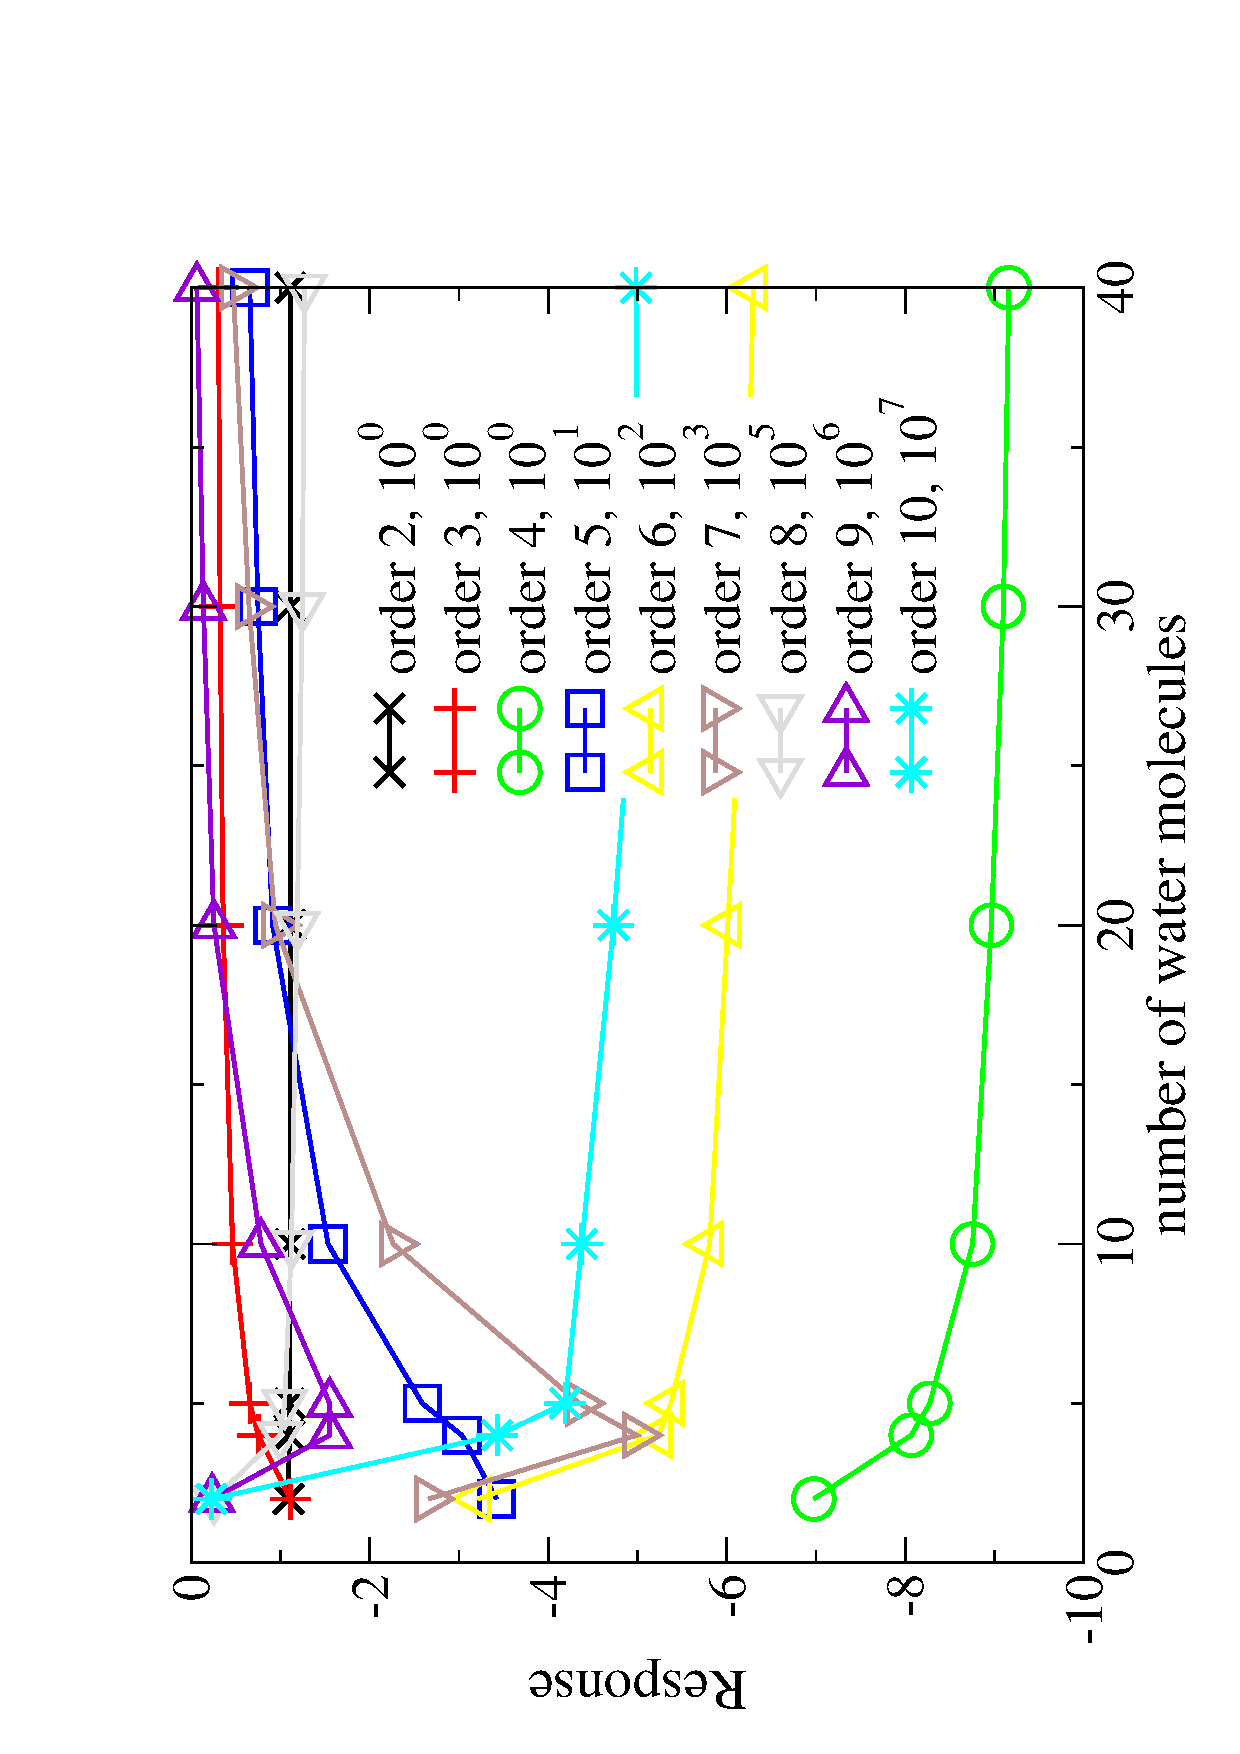
\includegraphics[angle=-90.00]{Order10}}
\end{figure}


\subsection{One dimensional water chains}
We have computed the (hyper)polarizabilities $\alpha_{zz}$, 
$\beta_{zzz}$ and $\gamma_{zzzz}$ of water oligomers containing
up to 20 water molecules. These calculations have been carried out at
both the RHF/6-31G level of
theory and at the {\tt GOOD} and {\tt TIGHT} thresholding parameters 
that control precision of the linear scaling algorithms.
The static properties of water chains have been evaluated
by using the same geometry as Otto {\em et al.} \cite{POtto99}. 
Our data is compared to polarizabilities
calculated with the GAMESS quantum chemistry package \cite{gamess} 
at the RHF/6-31G level of theory.  We also
present the results obtained with the density matrix 
based 2n+1 rule previously introduced.

\subsubsection{Numerical stability}

To investigate the numerical stability we compare the data calculated
with a {\tt TIGHT} numerical threshold ($10^{-6}$) with the polarizabilities
calculated using a {\tt GOOD} numerical threshold ($10^{-5}$). 
In tables \ref{tab:Alpha_1D_Values}-\ref{tab:Gamma_1D_Values} we find that
only 1-2 significant digit altered by reducing the threshold by two orders 
of magnitude. 

For example, a calculation of $(H_2O)_5$ with the {\tt VERYTIGHT} numerical threshold ($10^{-7}$) 
gives the following polarizabilities $\alpha_{zz}=6.822602\,a.u.$, $\beta_{zzz}=-19.892464\,a.u.$ and
$\gamma_{zzzz}=1168.95479\,a.u.$. We can conclude that the thresholds 
{\tt GOOD} and {\tt TIGHT} give approximatively 3-4 and 5-6 
correct digits respectivelly independently of the order of the response calculated.

The calculations of the first and second hyperpolarizabilities with the help of
the density matrix based $2n+1$ rule (See Tables \ref{tab:Beta_1D_Values} and \ref{tab:Gamma_1D_Values}) 
give about the same number of digit as the explicit calculations (i.e. 5-6 digits).

%vw\begin{figure}[t]
%vw  \caption{\protect
%vw    Longitudinal polarizability per water molecule
%vw    $\alpha_{zz}/N$ for 
%vw    the 6-31G and 6-31G** basis sets in function
%vw    of the number of water molecule in the chain.
%vw  }\label{fig:Alpha_1D}
%vw  \resizebox*{3.6in}{!}{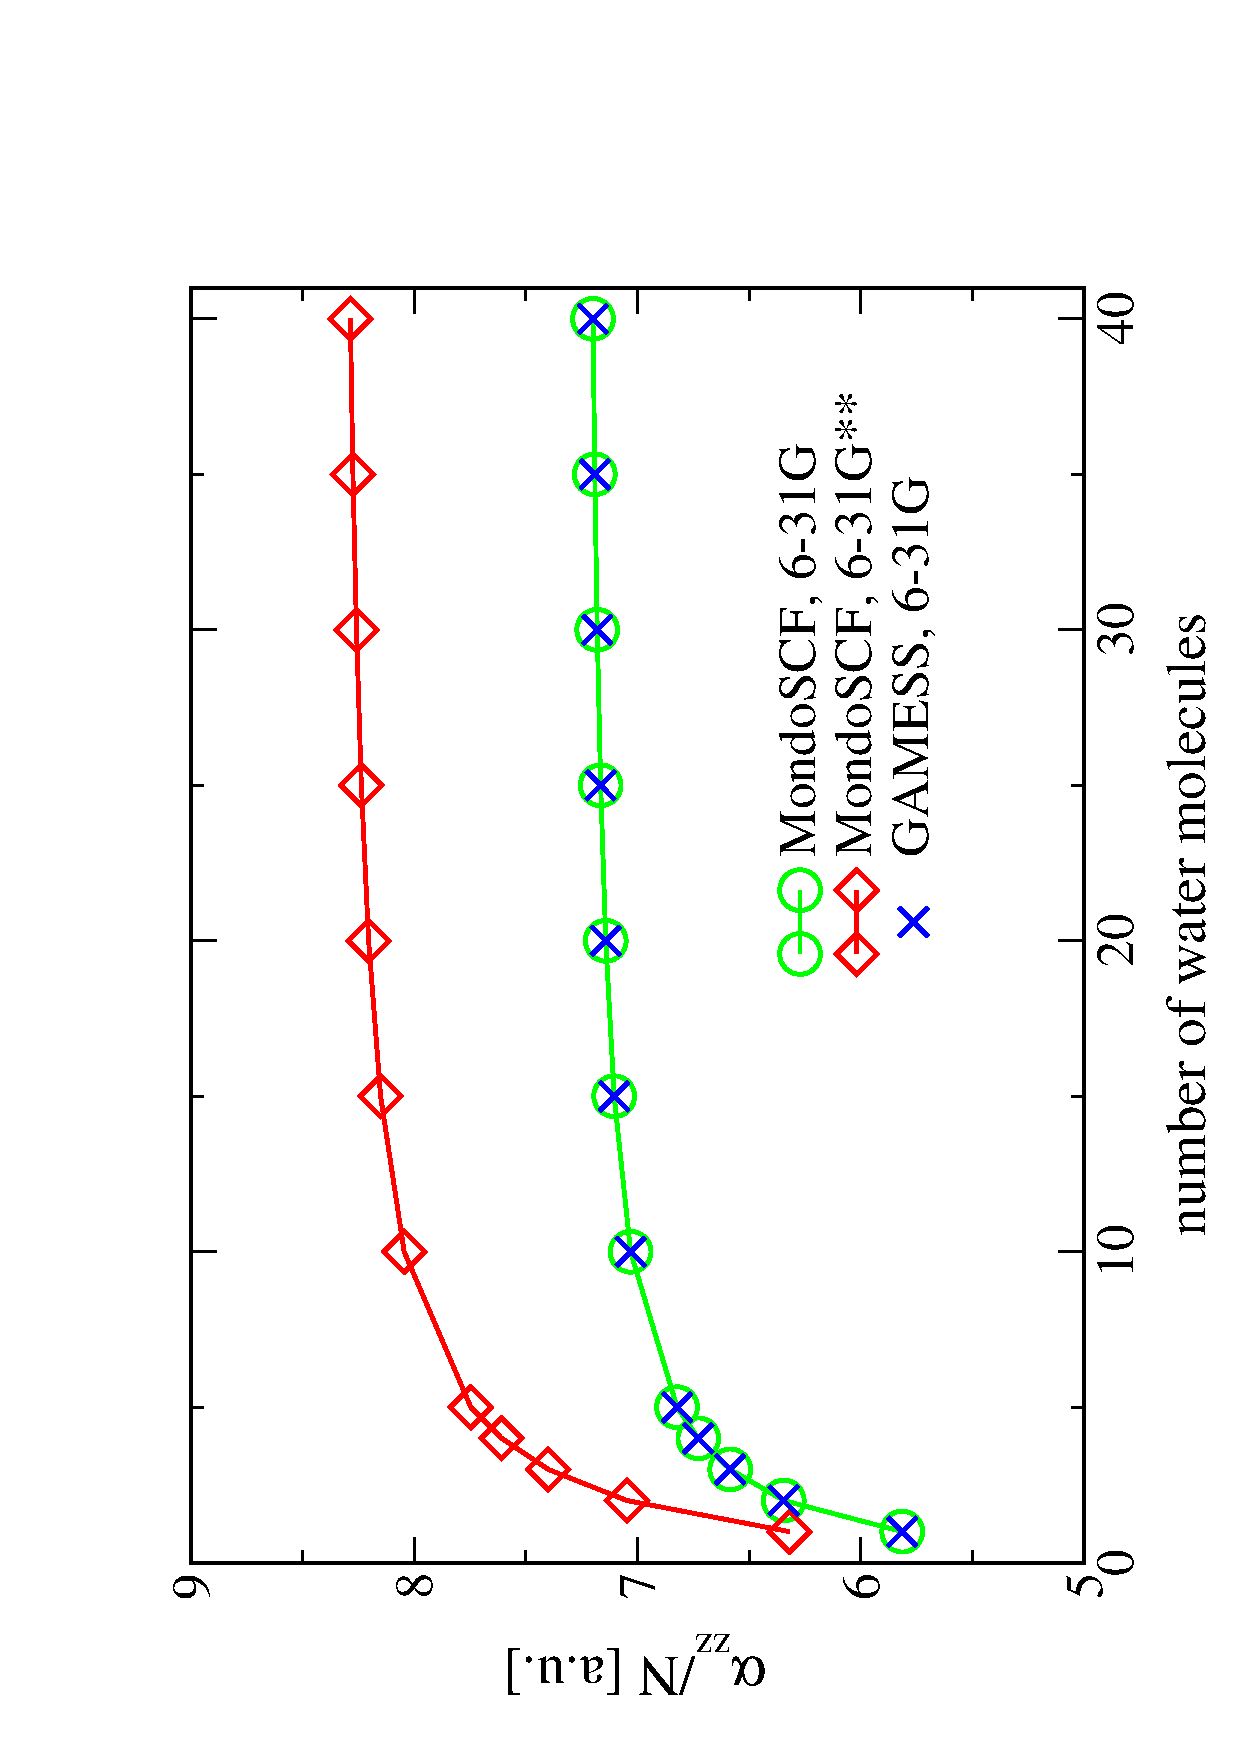
\includegraphics[angle=-90.00]{Alpha_all}}
%vw\end{figure}

%vw\begin{figure}[t]
%vw  \caption{\protect
%vw    Longitudinal first hyperpolarizability per water 
%vw    molecule $\beta_{zzz}/N$ for 
%vw    the 6-31G and 6-31G** basis sets in function
%vw    of the number of water molecule in the chain.
%vw  }\label{fig:Beta_1D}
%vw  \resizebox*{3.6in}{!}{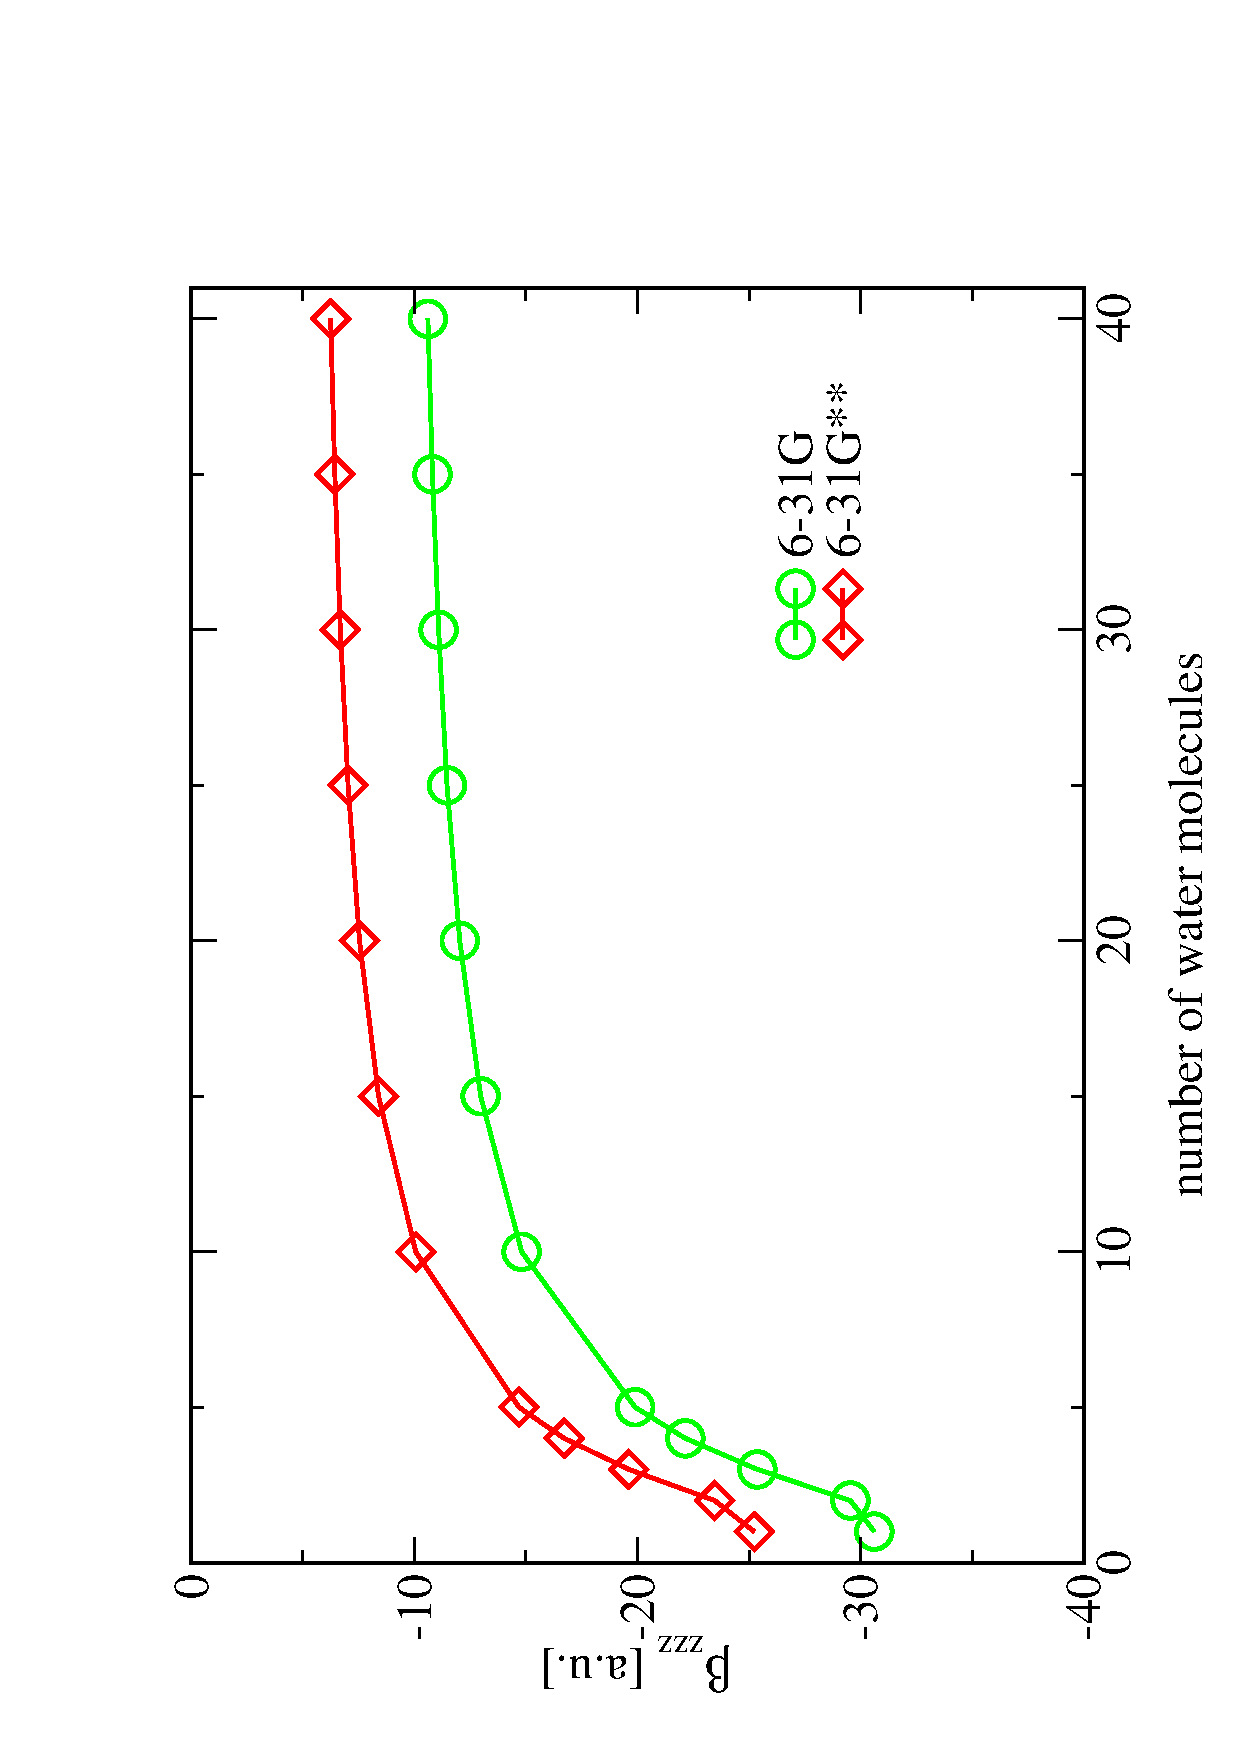
\includegraphics[angle=-90.00]{Beta_all}}
%vw\end{figure}

%vw\begin{figure}[t]
%vw  \caption{\protect
%vw    Longitudinal second hyperpolarizability per water
%vw    molecule $\gamma_{zzzz}/N$ for 
%vw    the 6-31G and 6-31G** basis sets in function
%vw    of the number of water molecule in the chain.
%vw  }\label{fig:Gamma_1D}
%vw  \resizebox*{3.6in}{!}{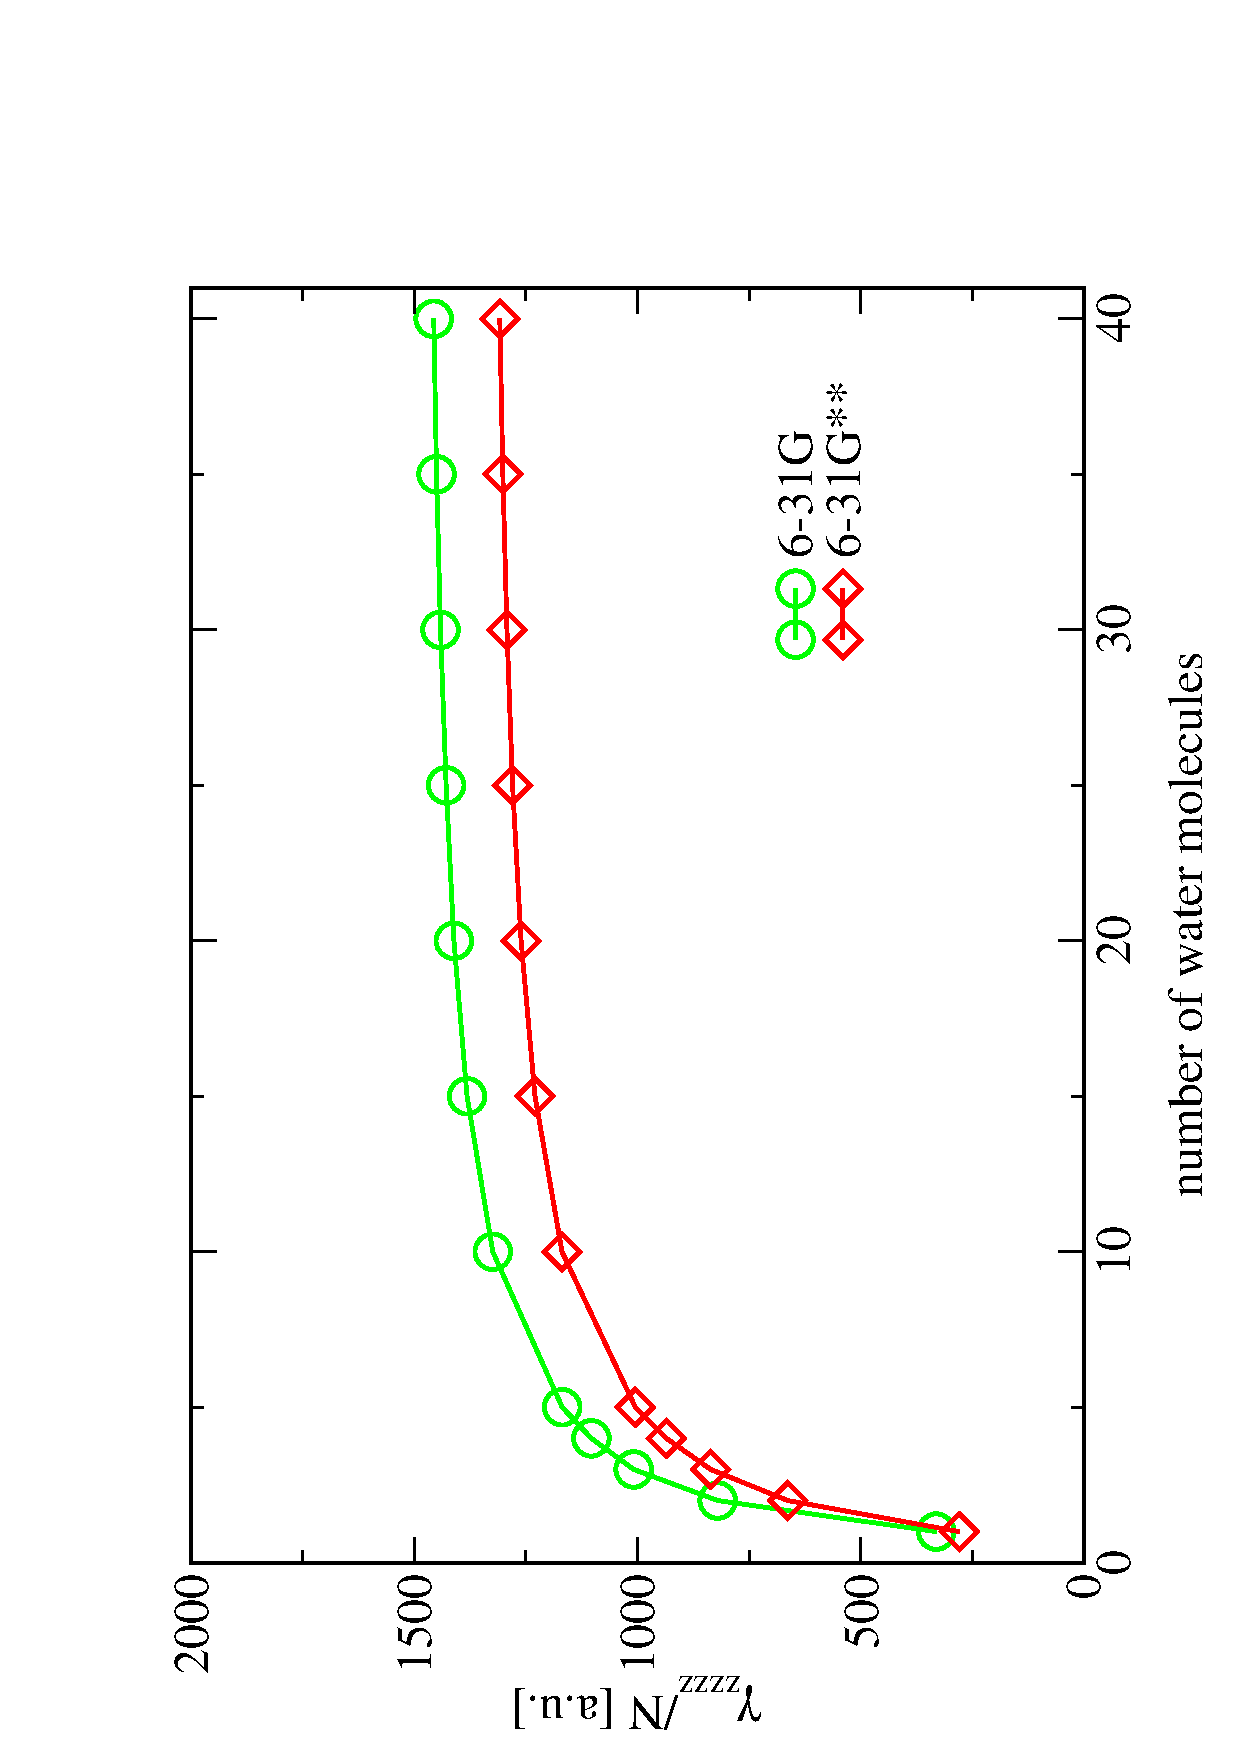
\includegraphics[angle=-90.00]{Gamma_all}}
%vw\end{figure}

\begin{table}[t]
  \centering
  \caption{\protect
    Longitudinal polarizability $\alpha_{zz}$
    for different water chain lengths with the 6-31G basis set
    and {\tt GOOD} and {\tt TIGHT} accuracies (See text) and the results obtained with
    the GAMESS quantum chemistry package \cite{gamess} with the 6-31G. 
    All the results are in $[a.u.]$.
  }\label{tab:Alpha_1D_Values}
  \begin{tabular}{cccc}
    \toprule
    $N$ &\multicolumn{1}{c}{{\sc GAMESS}}
        &\multicolumn{1}{c}{{\tt GOOD}}
        &\multicolumn{1}{c}{{\tt TIGHT}}\\
    \hline
     1 & 5.8136 & 5.817130 & 5.813589  \\
     2 & 6.3448 & 6.348235 & 6.344830  \\
     3 & 6.5844 & 6.585133 & 6.584449  \\
     4 & 6.7276 & 6.737545 & 6.727684  \\
     5 & 6.8226 & 6.823266 & 6.822640  \\
    10 & 7.0308 & 7.031487 & 7.030870  \\
    15 & 7.1047 & 7.105326 & 7.104780  \\
    20 & 7.1424 & 7.143081 & 7.142433  \\
%    25 & 7.1652 & - & 7.165231  \\
%    30 & 7.1805 & - & 7.180514  \\
%    35 & 7.1914 & - & 7.191468  \\
%    40 & 7.1996 & - & 7.199704  \\
    \botrule
  \end{tabular}
\end{table}


\begin{table}
  \centering
  \caption{\protect
    Longitudinal first hyperpolarizability $\beta_{zzz}$
    for different water chain lengths with the 6-31G basis set
    and {\tt GOOD} and {\tt TIGHT} accuracies (See text) and the results obtained with
    the GAMESS quantum chemistry package \cite{gamess} with the 6-31G. 
    All the results are in $[a.u.]$.
  }\label{tab:Beta_1D_Values}
  \begin{tabular}{ccccc}
    \toprule
    $N$ &\multicolumn{1}{c}{{\sc GAMESS}}
    &\multicolumn{1}{c}{{\tt GOOD}}
    &\multicolumn{1}{c}{{\tt TIGHT}}
    &\multicolumn{1}{c}{{\tt TIGHT}\footnote[1]{The density matrix based 2n+1 rule has been used.}} \\
    \hline
     1 & -30.6125 & -30.612180 & -30.612178 & -30.612274  \\
     2 & -29.5444 & -29.555935 & -29.545096 & -29.545207  \\
     3 & -25.3696 & -25.382010 & -25.370516 & -25.370628  \\
     4 & -22.1411 & -22.147670 & -22.141553 & -22.141869  \\
     5 & -19.8925 & -19.903268 & -19.893306 & -19.893441  \\
    10 & -14.8063 & -14.815886 & -14.807203 & -14.807392  \\
    15 & -12.9713 & -12.978256 & -12.972171 & -12.972379  \\
    20 & -12.0334 & -12.038114 & -12.034259 & -12.034505  \\
%    25 & -11.4648 & - & -11.465624 & -11.465915  \\
%    30 & -11.0834 & - & -11.084234 & -11.084569  \\
%    35 & -10.8099 & - & -10.810645 & -10.811061  \\
%    40 & -10.6042 & - & -10.604860 & -10.605360  \\
    \botrule
  \end{tabular}
\end{table}

\begin{table}
  \centering
  \caption{\protect
    Longitudinal second hyperpolarizability $\gamma_{zzzz}$
    for different water chain lengths with the 6-31G basis set
    and {\tt GOOD} and {\tt TIGHT} accuracies (See text) and the results obtained with
    the GAMESS quantum chemistry package \cite{gamess} with the 6-31G. 
    All the results are in $[a.u.]$.
  }\label{tab:Gamma_1D_Values}
  \begin{tabular}{ccccc}
    \toprule
    $N$ &\multicolumn{1}{c}{{\sc GAMESS}}
    &\multicolumn{1}{c}{{\tt GOOD}}
    &\multicolumn{1}{c}{{\tt TIGHT}}
    &\multicolumn{1}{c}{{\tt TIGHT}\footnote[1]{The density matrix based 2n+1 rule has been used.}} \\
    \hline
     1 &  330.5753 &  330.545460 &  330.577009 &  330.572592 \\
     2 &  820.1398 &  820.448185 &  820.160650 &  820.153734 \\
     3 & 1008.5656 & 1008.894703 & 1008.580733 & 1008.582556 \\
     4 & 1103.4813 & 1103.793125 & 1103.494950 & 1103.497148 \\
     5 & 1168.9563 & 1169.325236 & 1168.972479 & 1168.975145 \\
    10 & 1324.2906 & 1325.421145 & 1324.304700 & 1324.307818 \\
    15 & 1381.8657 & 1383.380593 & 1381.882600 & 1381.882180 \\
    20 & 1411.4264 & 1414.736619 & 1411.448699 & 1411.437607 \\
%    25 & 1429.3767 & - & 1428.980999 & 1429.379837 \\
%    30 & 1441.4261 & - & 1441.474333 & 1441.418800 \\
%    35 & 1450.0713 & - & 1450.143685 & 1450.043351 \\
%    40 & 1456.5756 & - & 1456.682800 & 1456.520170 \\
    \botrule
  \end{tabular}
\end{table}

\subsection{Linear scaling: 3D water clusters}

In Figs \ref{fig:Alpha_scaling}-\ref{fig:Gamma_scaling} the total CPU time for 
the fifth CPSCF cycle (including build time
for $\F^{a\ldots}$, iterative construction of $\D^{a\ldots}$ and all intermadiate
steps including the congruence tranformation) for the first, second and third
order, repectively, are shown for the RHF/6-31G and RHF/6-31G** levels of
theory and at both the {\tt GOOD} and {\tt TIGHT} thresholding parameter 
sets that control precision of the linear scaling algorithms, corresponding 
to matrix thresholds of $10^{-5}$ and $10^{-6}$, respectively. The convergence
of the CPSCF equations is typically achived in about 10 cycles, independent of the
cluster size, basis set, matrix threshold or order of the response calculated.

The 3D water clusters show an early onset of linear scaling for accurate
basis set, low thresholds and high order response.
Thus, the second order response Fig. \ref{fig:Beta_scaling} shows a linear scaling
onset as early as the first order response e.g. about 70 water molecules at
the RHF/6-31G level of theory and {\tt GOOD} threshold. In the case of the third order
response, the $\mathcal{O}(N)$ behavior comes to light at about 90 water 
molecules for the small basis set (6-31G) and {\tt GOOD}. 
To appreciate the difference in computational time between each order,
we have plotted in Figure \ref{fig:Mix_scaling} the total CPU time for the
first, second and third order CPSCF cycle at the RHF/6-31G level of theory and {\tt TIGHT}. 
In the linear scaling regime, we can observe a timing ratio, relatively to first order, 
of $1.5$ and $2.2$ for the second and third order respectively.

\subsubsection{Exponential decay}
Figure \ref{fig:Superposition_Decay} shows the superposition 
of the magnitude of density matrix derivative atom-atom blocks up to 
third order as a function of atom-atom distance when perturbed by 
a static electric field. 
The density responses matrices show an exponential decay as a function
of the internuclear distance, however the decay is slower and the locality
becomes lower for the higher order response functions.
Therefore, we find a later onset for the linear scaling for the higher order
responses. 


\subsubsection{Onset of linear scaling}

To analyse more into detail the linear scaling behavior of the third order
response, we have plotted in Figs. \ref{fig:Gamma_QCTC_Timing}-\ref{fig:Gamma_ONX_Timing} 
the CPU time for the three most consuming parts of a CPSCF step, i.e. the Coulomb matrix, 
the perturbed density matrix build and the exchange matrix respectively. 
The dominating critical part of each calculation is found to scale linearly
in computational complexity for each individual subset of the computation. 

%\subsubsection{QCTC}
In case of the Coulomb build Figure \ref{fig:Gamma_QCTC_Timing}, 
the linear scaling arises as early as 30 water molecules for the 
{\tt GOOD} threshold and about 50 molecules for the
{\tt TIGHT} threshold. As we use a localized basis function the 
Hermit-Gaussian density can be built in a $\mathcal{O}(N)$ fashion....


%\subsubsection{TC2}
In the perturbed density build, the $\mathcal{O}(N)$ behavior is obtained
between 70 to 110 water molecules depanding on the threshold 
Figure~\ref{fig:Gamma_TC2R_Timing}. The $\mathcal{O}(N)$ scaling results 
from the fact that the matrix multiplications, in the purification
scheme, always happen as $\X^{abc}_i\X^{0}_i$ or $\X^{ab}_i\X^{c}_i$
which is a dense matrix multiply by a sparser matrix.

%\subsubsection{ONX}
The exchange matrix build is dominated by a linear term which has a high prefactor, thus
masking the non-linear terms.


\begin{figure}[t]
  \caption{\protect
    Total CPU time of the fifth first order CPSCF iteration for
    the water cluster sequence with the 6-31G and 6-31G** 
    basis sets and the {\tt GOOD} and {\tt TIGHT} 
    numerical thresholds (see text) controlling numerical
    precision of the result. The lines are fits to the 
    last three and four points, respectively.
  }\label{fig:Alpha_scaling}
  \resizebox*{3.6in}{!}{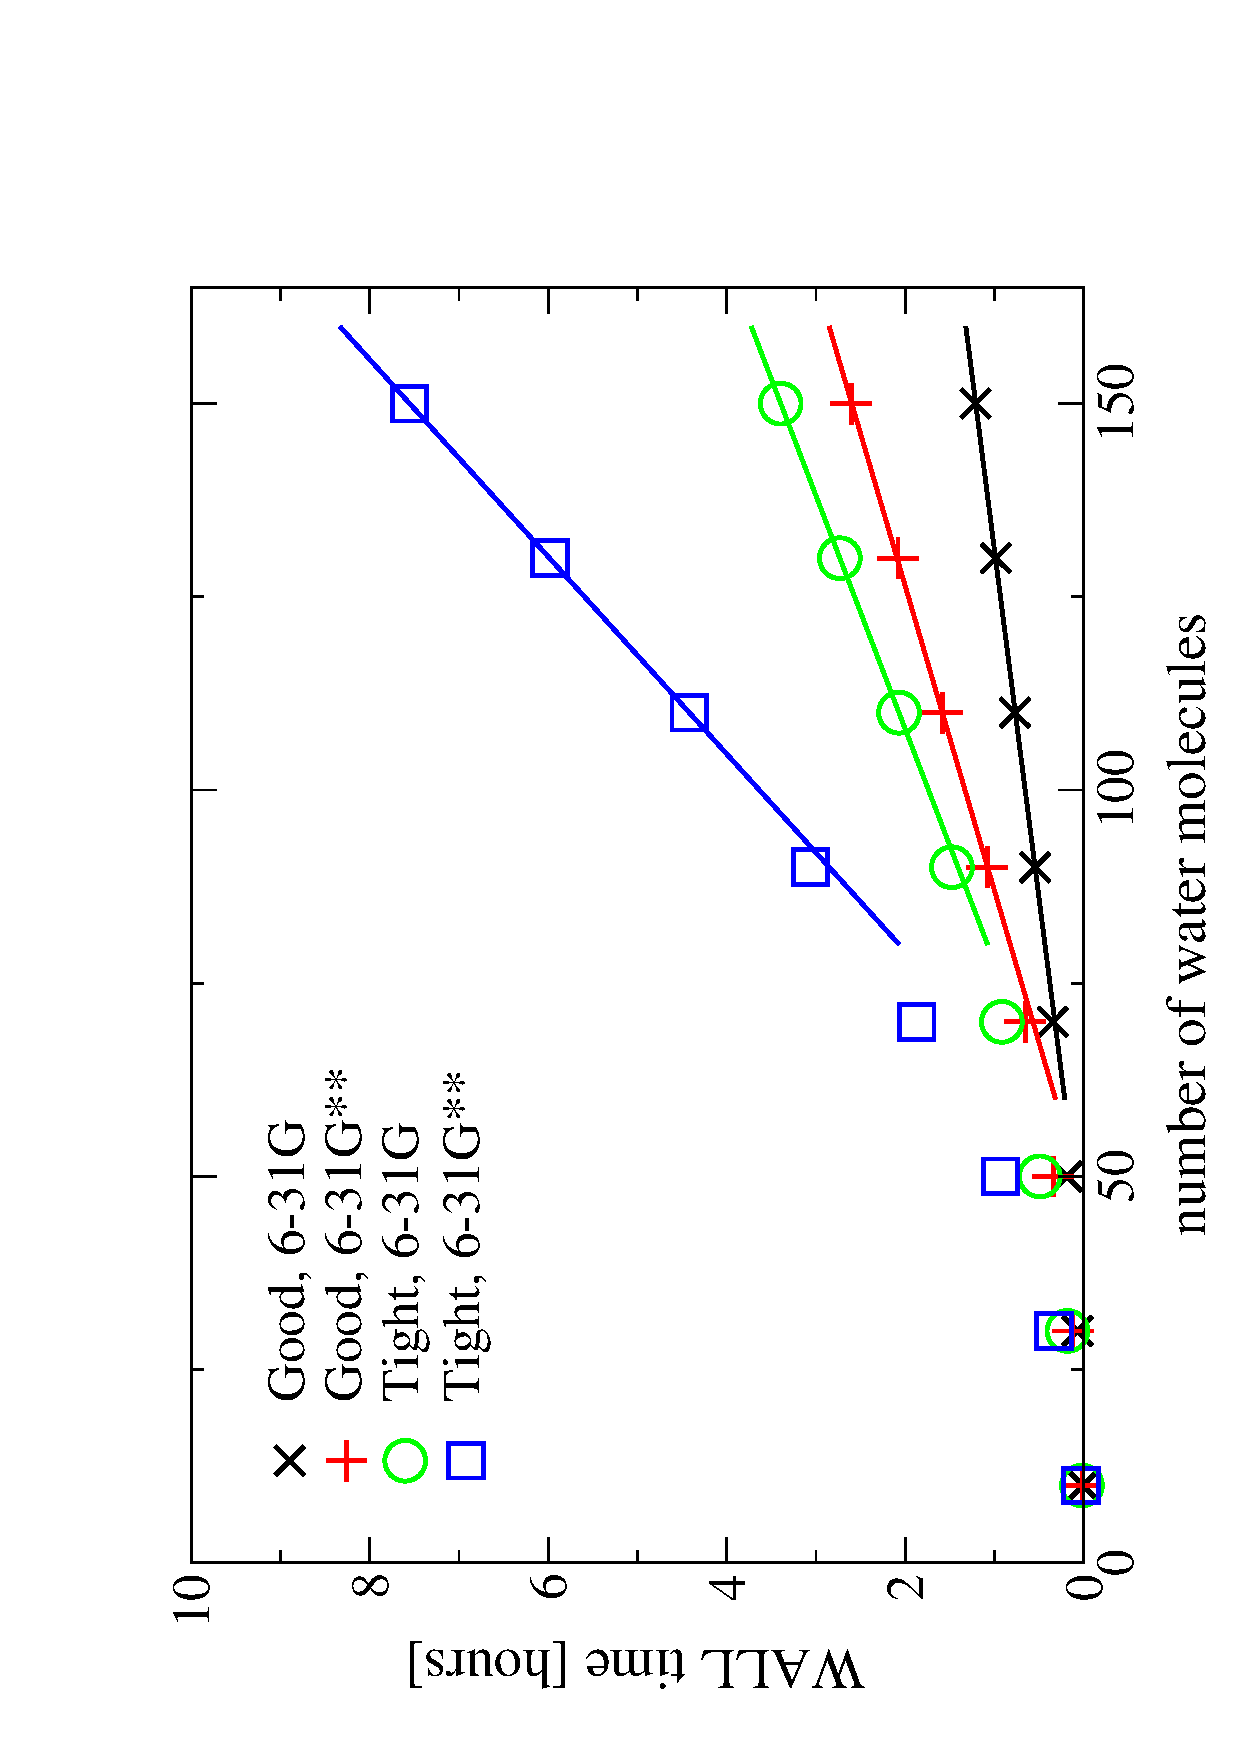
\includegraphics[angle=-90.00]{Alpha_h2o3D_6-31G_6-31Gss_G_T}}
\end{figure}


\begin{figure}[t]
  \caption{\protect
    Total CPU time of the fifth second order CPSCF iteration for
    the water cluster sequence with the 6-31G and 6-31G** 
    basis sets and the {\tt GOOD} and {\tt TIGHT} 
    numerical thresholds (see text) controlling numerical
    precision of the result. The lines are fits to the 
    last three and four points, respectively.
  }\label{fig:Beta_scaling}
  \resizebox*{3.6in}{!}{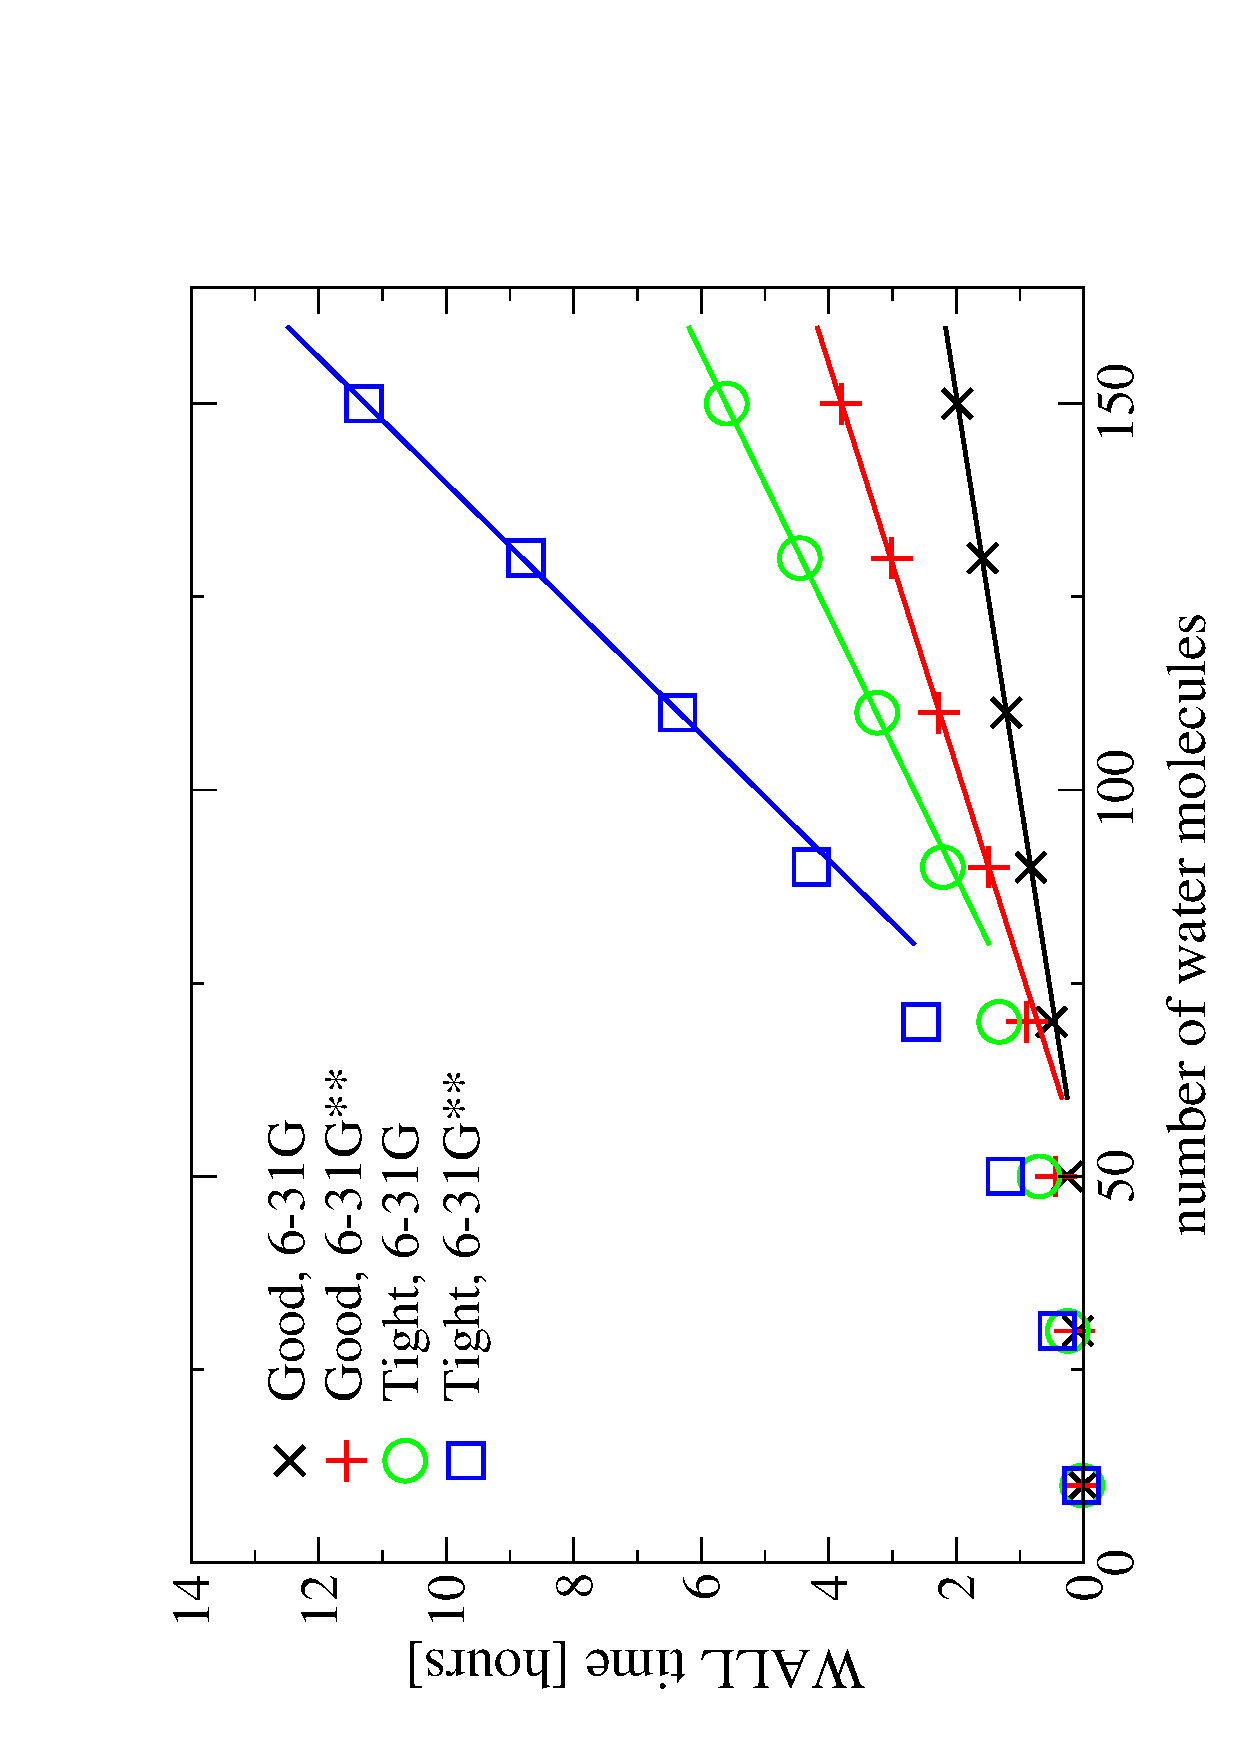
\includegraphics[angle=-90.00]{Beta_h2o3D_6-31G_6-31Gss_G_T}}
\end{figure}

\begin{figure}[t]
  \caption{\protect
    Total CPU time of the fifth third order CPSCF iteration for
    the water cluster sequence with the 6-31G and 6-31G** 
    basis sets and the {\tt GOOD} and {\tt TIGHT} 
    numerical thresholds (see text) controlling numerical
    precision of the result. The lines are fits to the 
    last three and four points, respectively.
  }\label{fig:Gamma_scaling}
  \resizebox*{3.6in}{!}{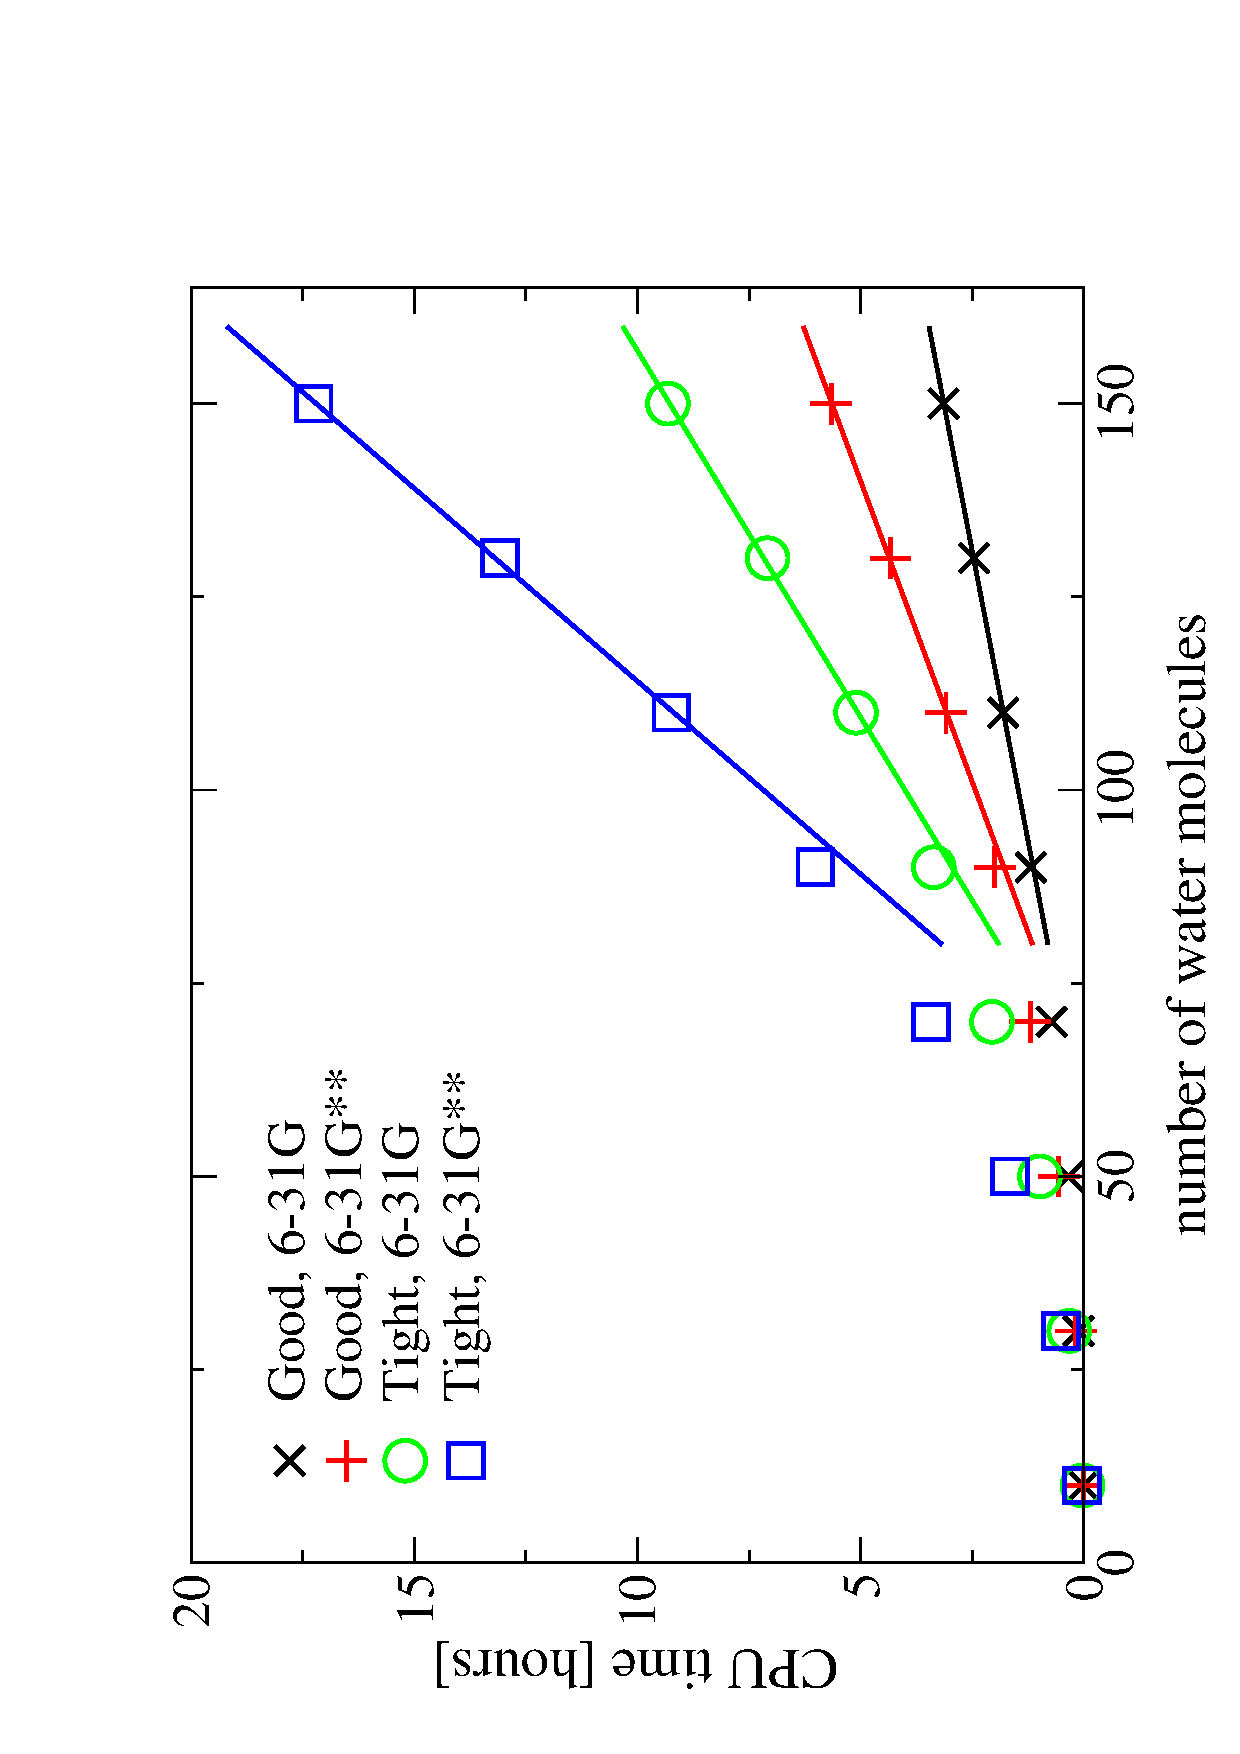
\includegraphics[angle=-90.00]{Gamma_h2o3D_6-31G_6-31Gss_G_T}}
\end{figure}

\begin{figure}[t]
  \caption{\protect
    Total CPU time of the fifth CPSCF iteration of first, second 
    and third order for the water cluster sequence with the 6-31G
    basis set and the {\tt TIGHT} numerical threshold (see text) 
    controlling numerical precision of the result. The lines
    are fits to the last three and four points, respectively.
  }\label{fig:Mix_scaling}
  \resizebox*{3.6in}{!}{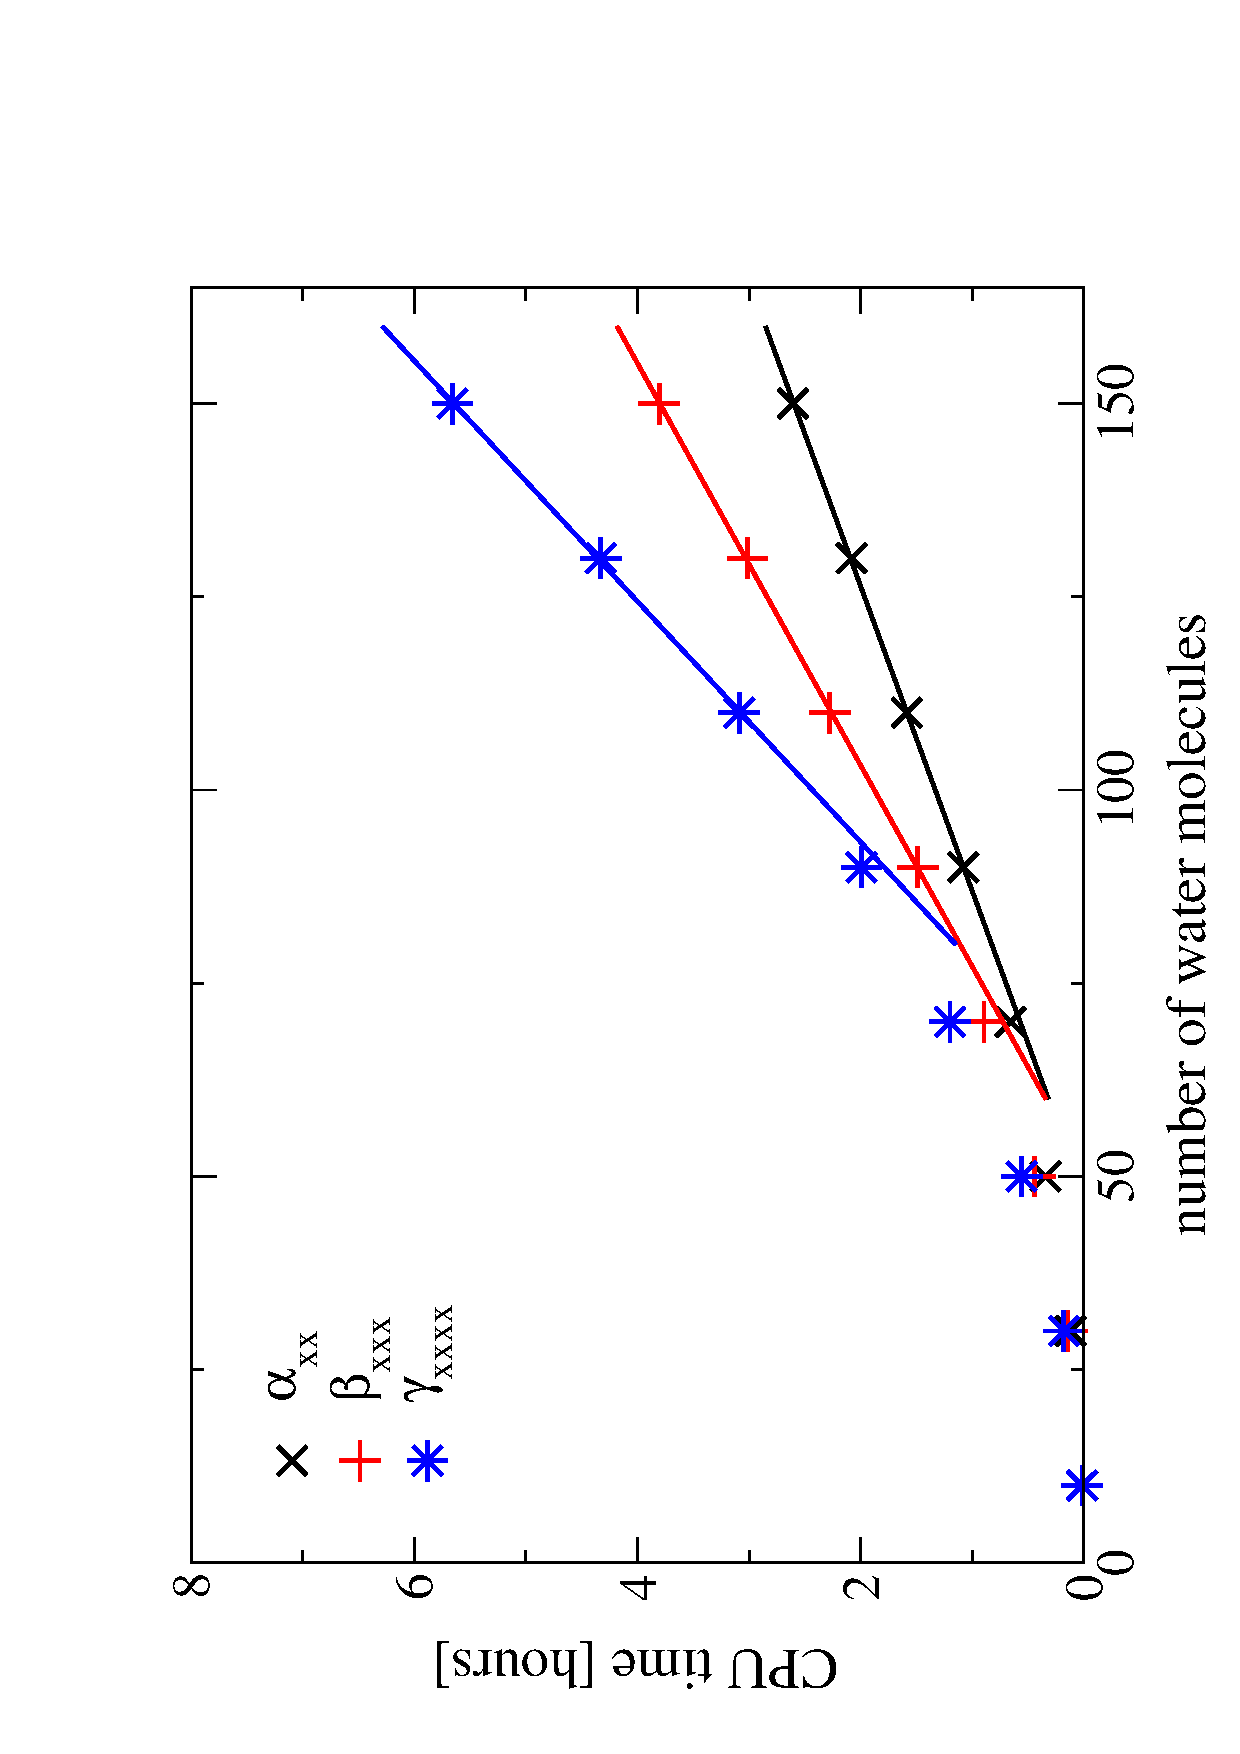
\includegraphics[angle=-90.00]{Mix_h2o3D_6-31G_T}}
\end{figure}

\begin{figure}[t]
  \caption{\protect
    QCTC CPU time of the fifth CPSCF iteration of third order for
    the water cluster sequence with the 6-31G and 6-31G** 
    basis sets and the {\tt GOOD} and {\tt TIGHT} 
    numerical thresholds (see text) controlling numerical
    precision of the result. The lines are fits to the 
    last three and four points, respectively.
  }\label{fig:Gamma_QCTC_Timing}
  \resizebox*{3.6in}{!}{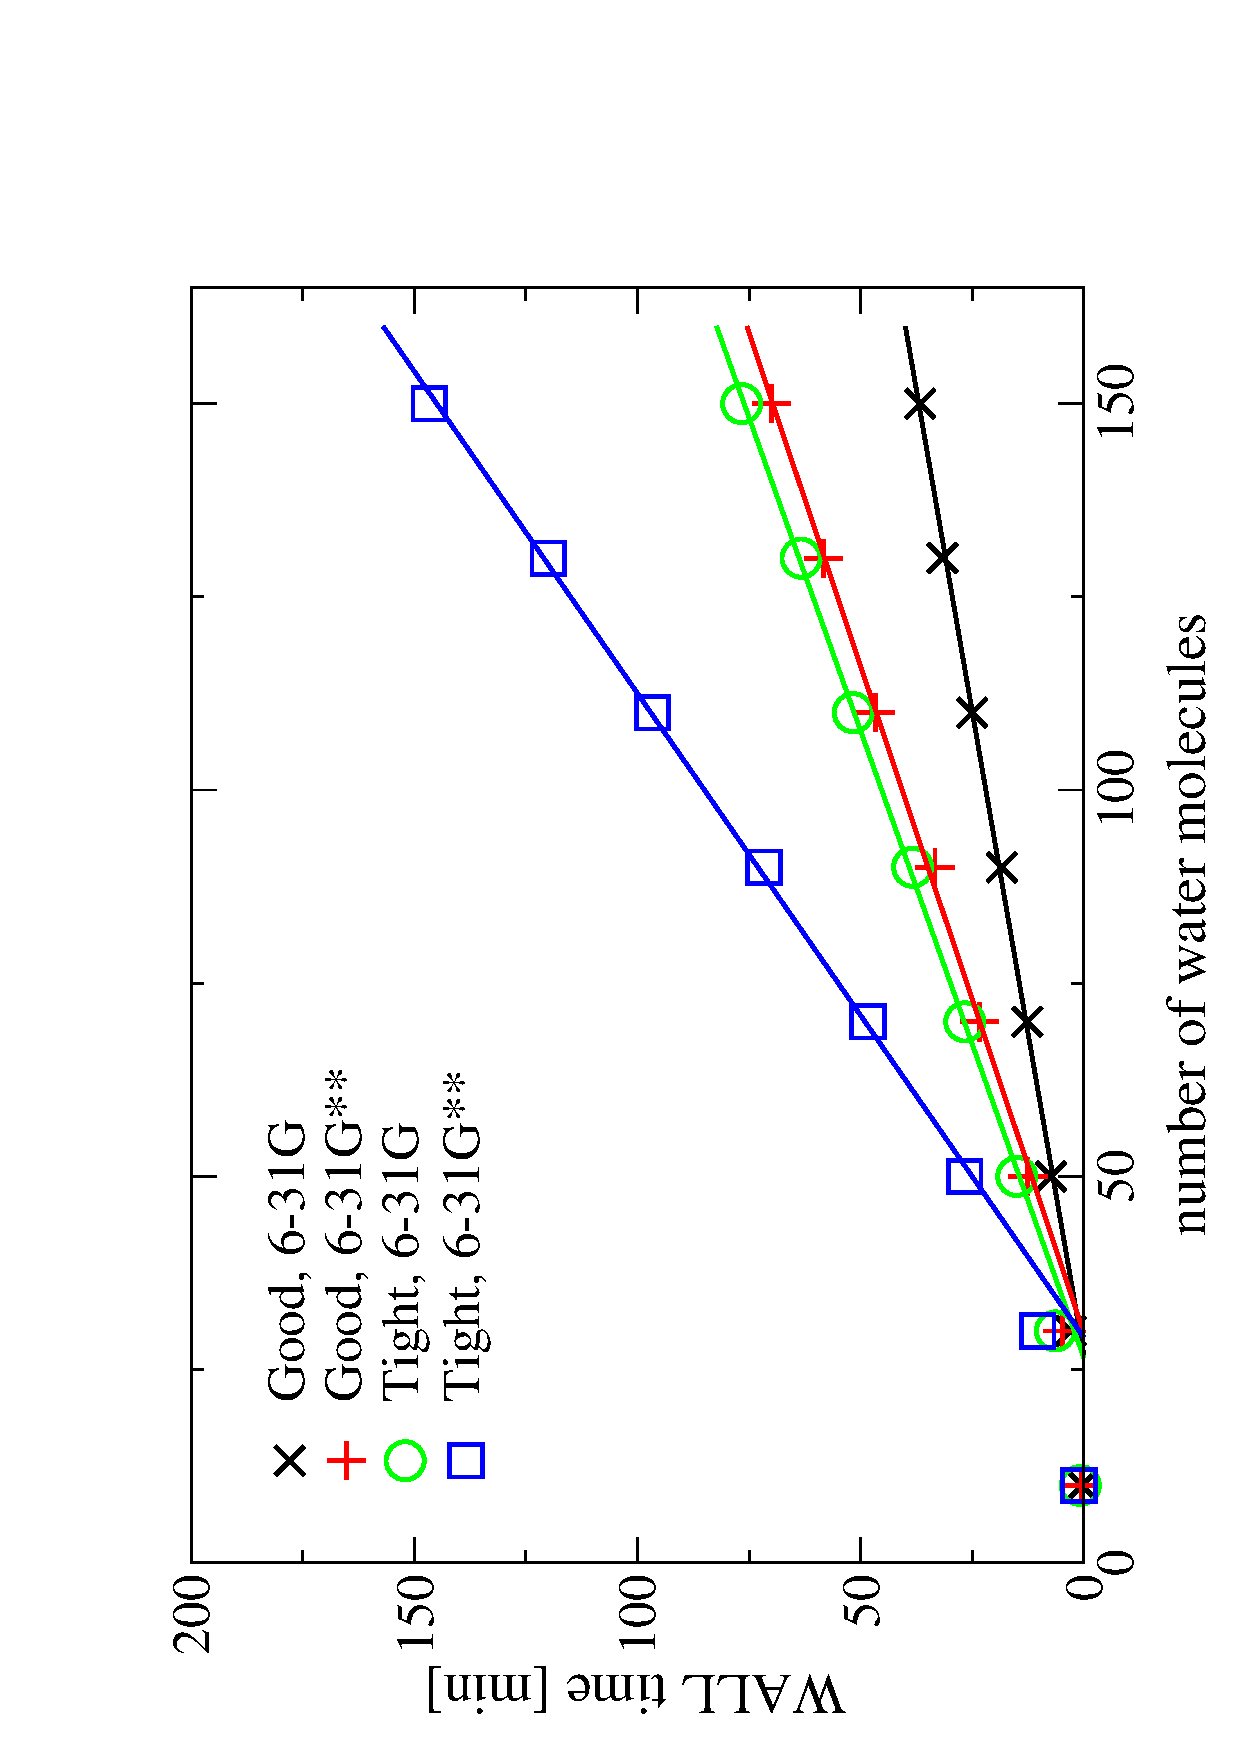
\includegraphics[angle=-90.00]{Gamma_QCTC_T}}
\end{figure}

\begin{figure}[t]
  \caption{\protect
    TC2R {\bf TC2R not explained?} CPU time of the fifth CPSCF iteration of third order for
    the water cluster sequence with the 6-31G and 6-31G** 
    basis sets and the {\tt GOOD} and {\tt TIGHT} 
    numerical thresholds (see text) controlling numerical
    precision of the result. The lines are fits to the 
    last three and four points, respectively.
  }\label{fig:Gamma_TC2R_Timing}
  \resizebox*{3.6in}{!}{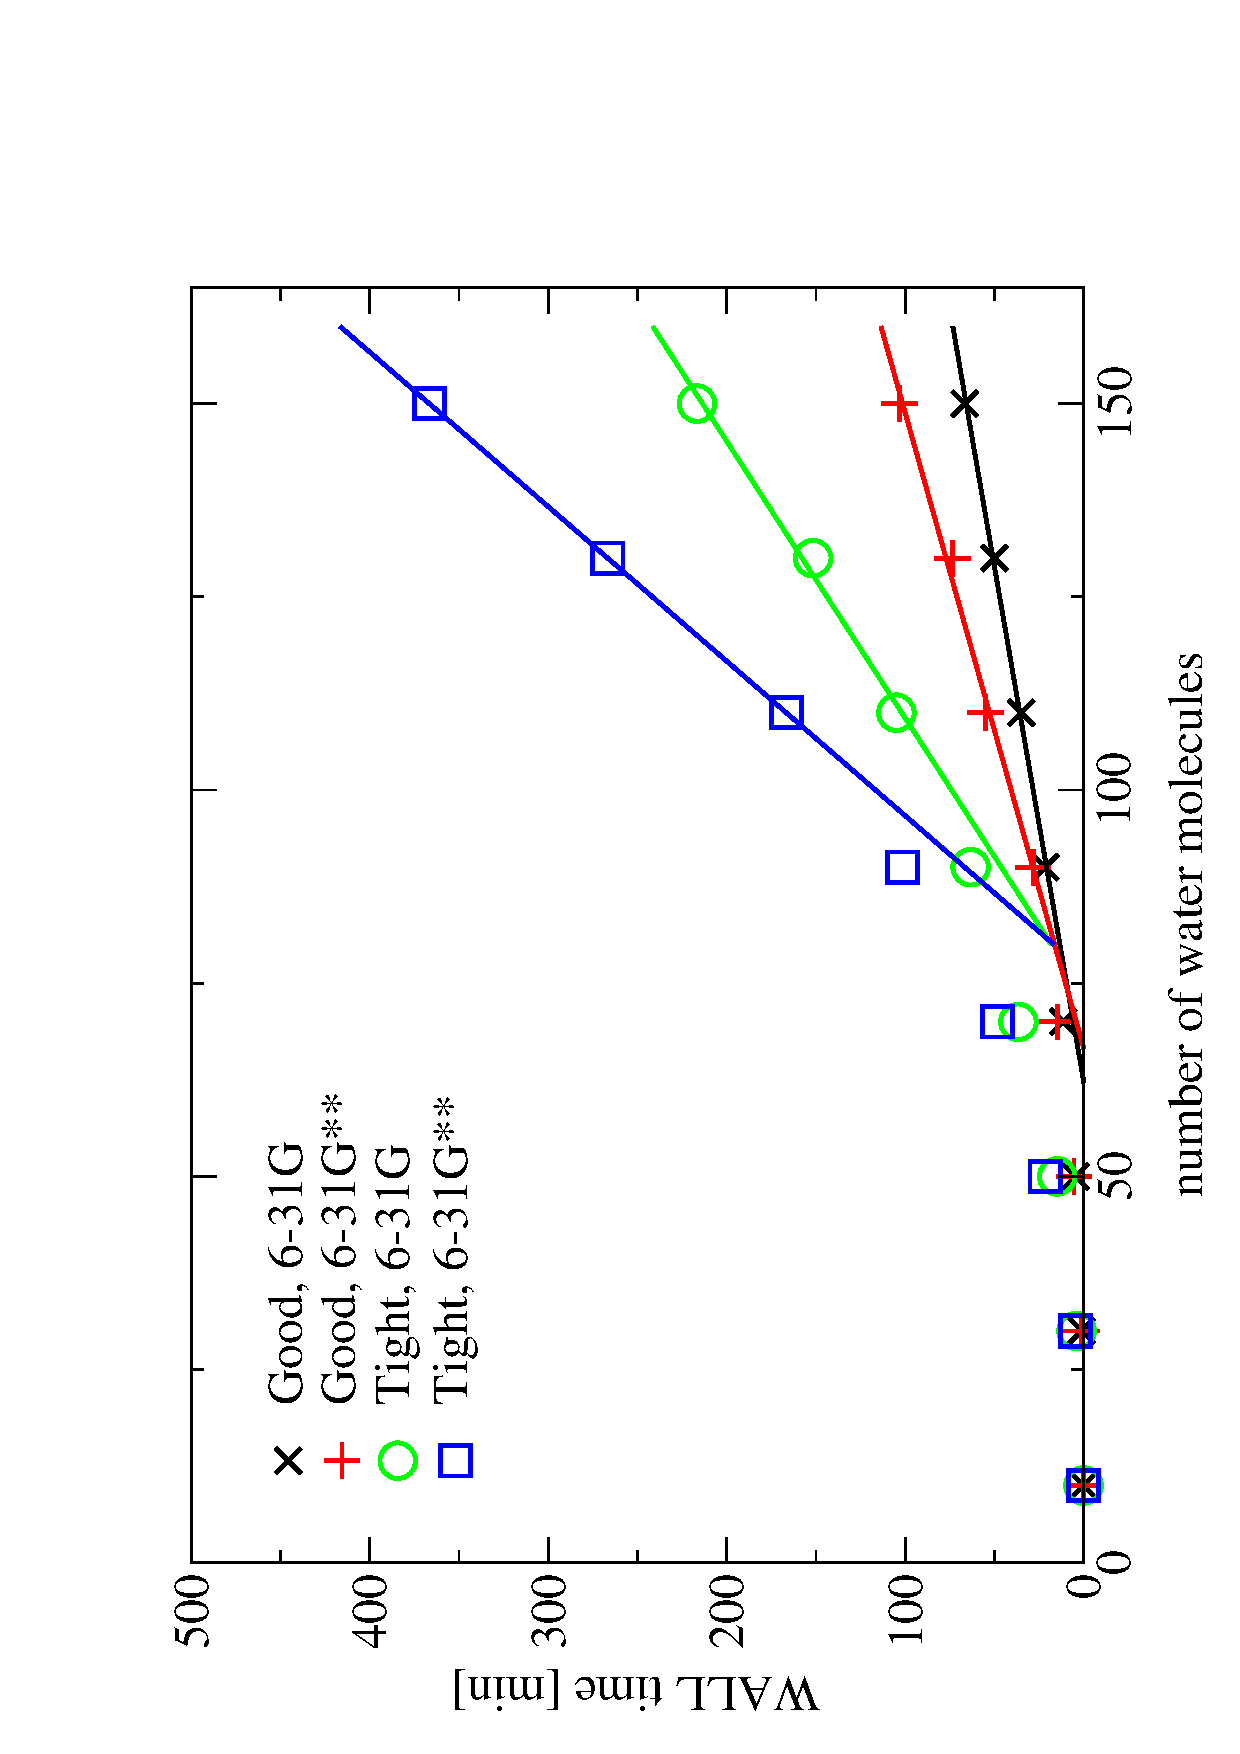
\includegraphics[angle=-90.00]{Gamma_TC2R_T}}
\end{figure}

\begin{figure}[t]
  \caption{\protect
    ONX CPU time of the fifth CPSCF iteration of third order for
    the water cluster sequence with the 6-31G and 6-31G** 
    basis sets and the {\tt GOOD} and {\tt TIGHT} 
    numerical thresholds (see text) controlling numerical
    precision of the result. The lines are fits to the 
    last three and four points, respectively.
  }\label{fig:Gamma_ONX_Timing}
  \resizebox*{3.6in}{!}{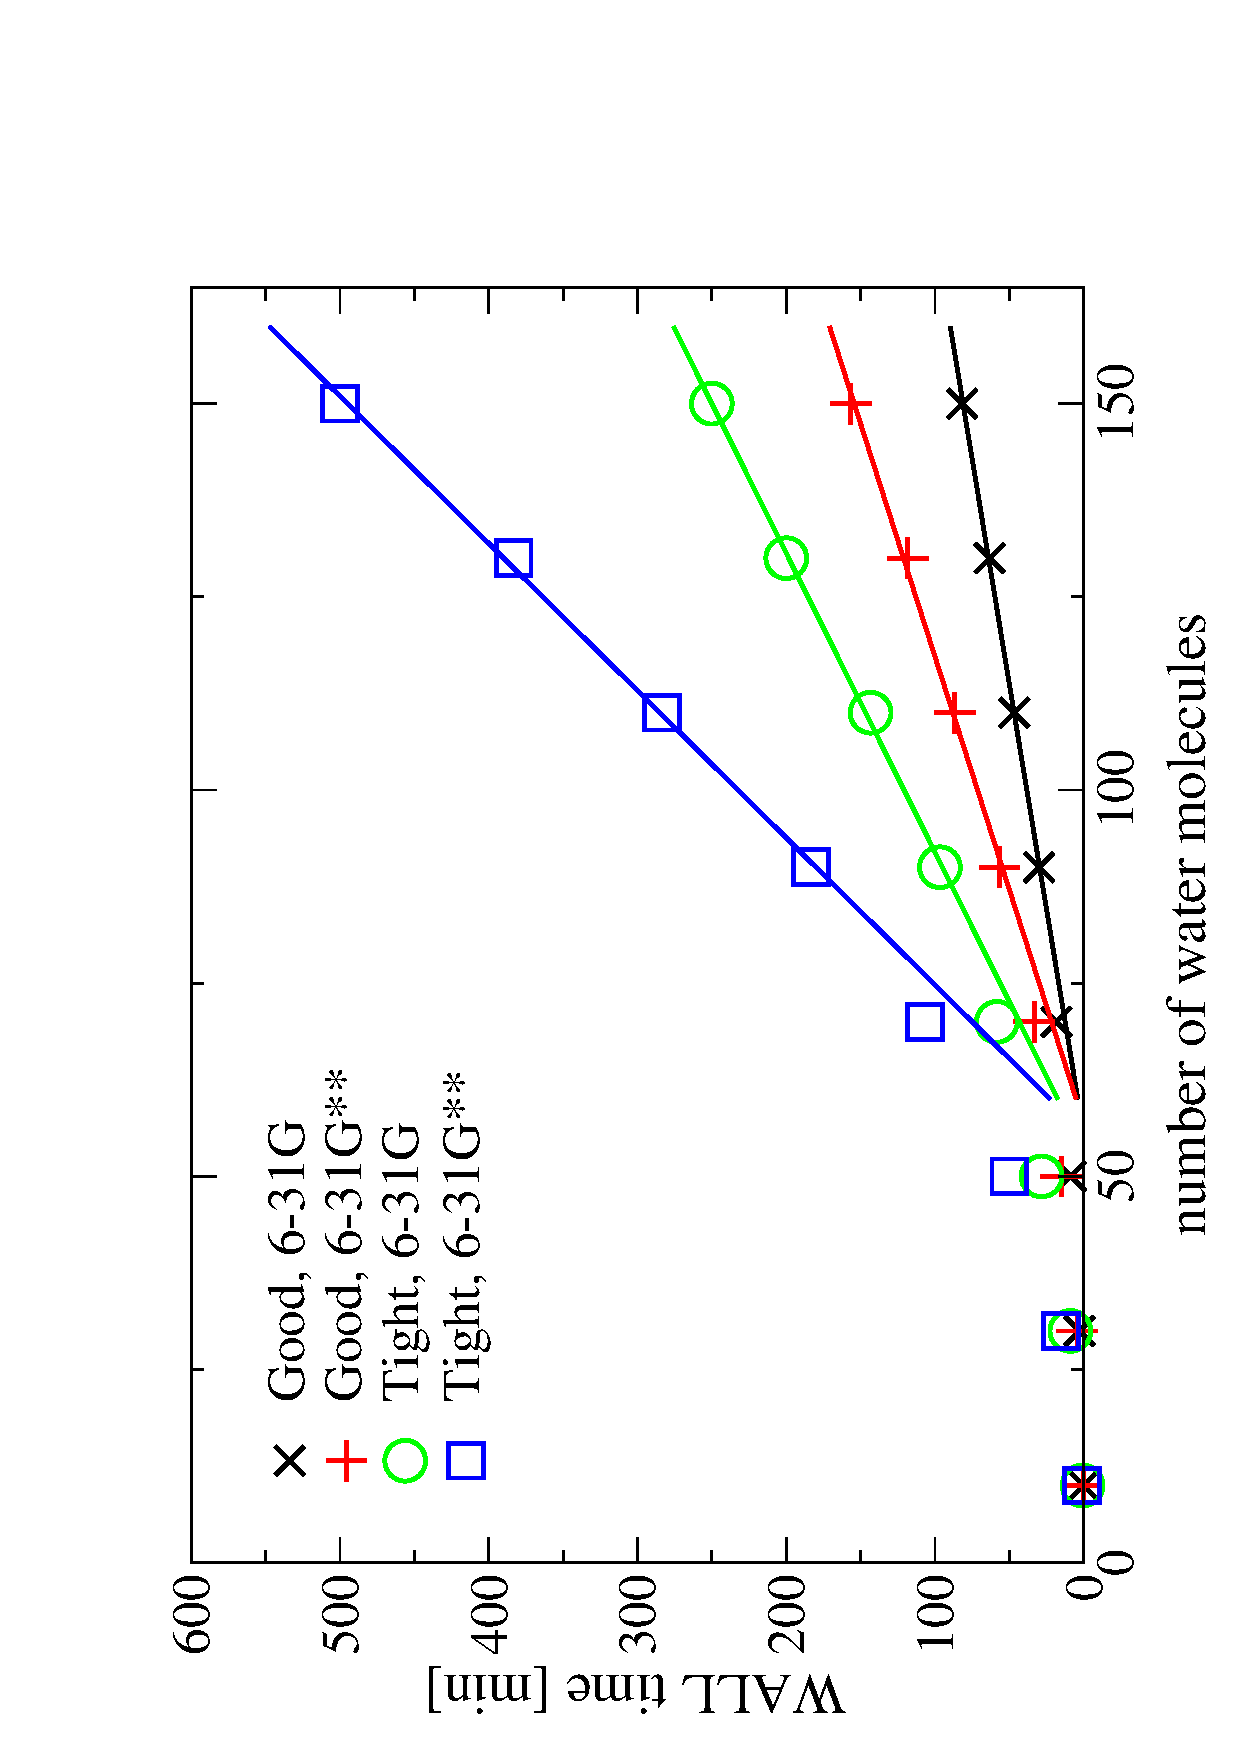
\includegraphics[angle=-90.00]{Gamma_ONX_T}}
\end{figure}

\begin{figure}[t]
  \caption{\protect
    Superposition of the magnitudes of the RHF/6-31G density matrix
    derivative elements $D_{cd}$, $D^{x}_{cd}$, $D^{xx}_{cd}$ and $D^{xxx}_{cd}$
    along the $x$ axis with the separation of basis function centers
    for the $\rm (H_2O)_{150}$ water cluster. The density matrix 
    derivatives have been converged to within {\tt TIGHT} (e.g. 
    matrix threshold of $10^{-6}$ $[a.u.]$).
  }\label{fig:Superposition_Decay}
  \resizebox*{3.6in}{!}{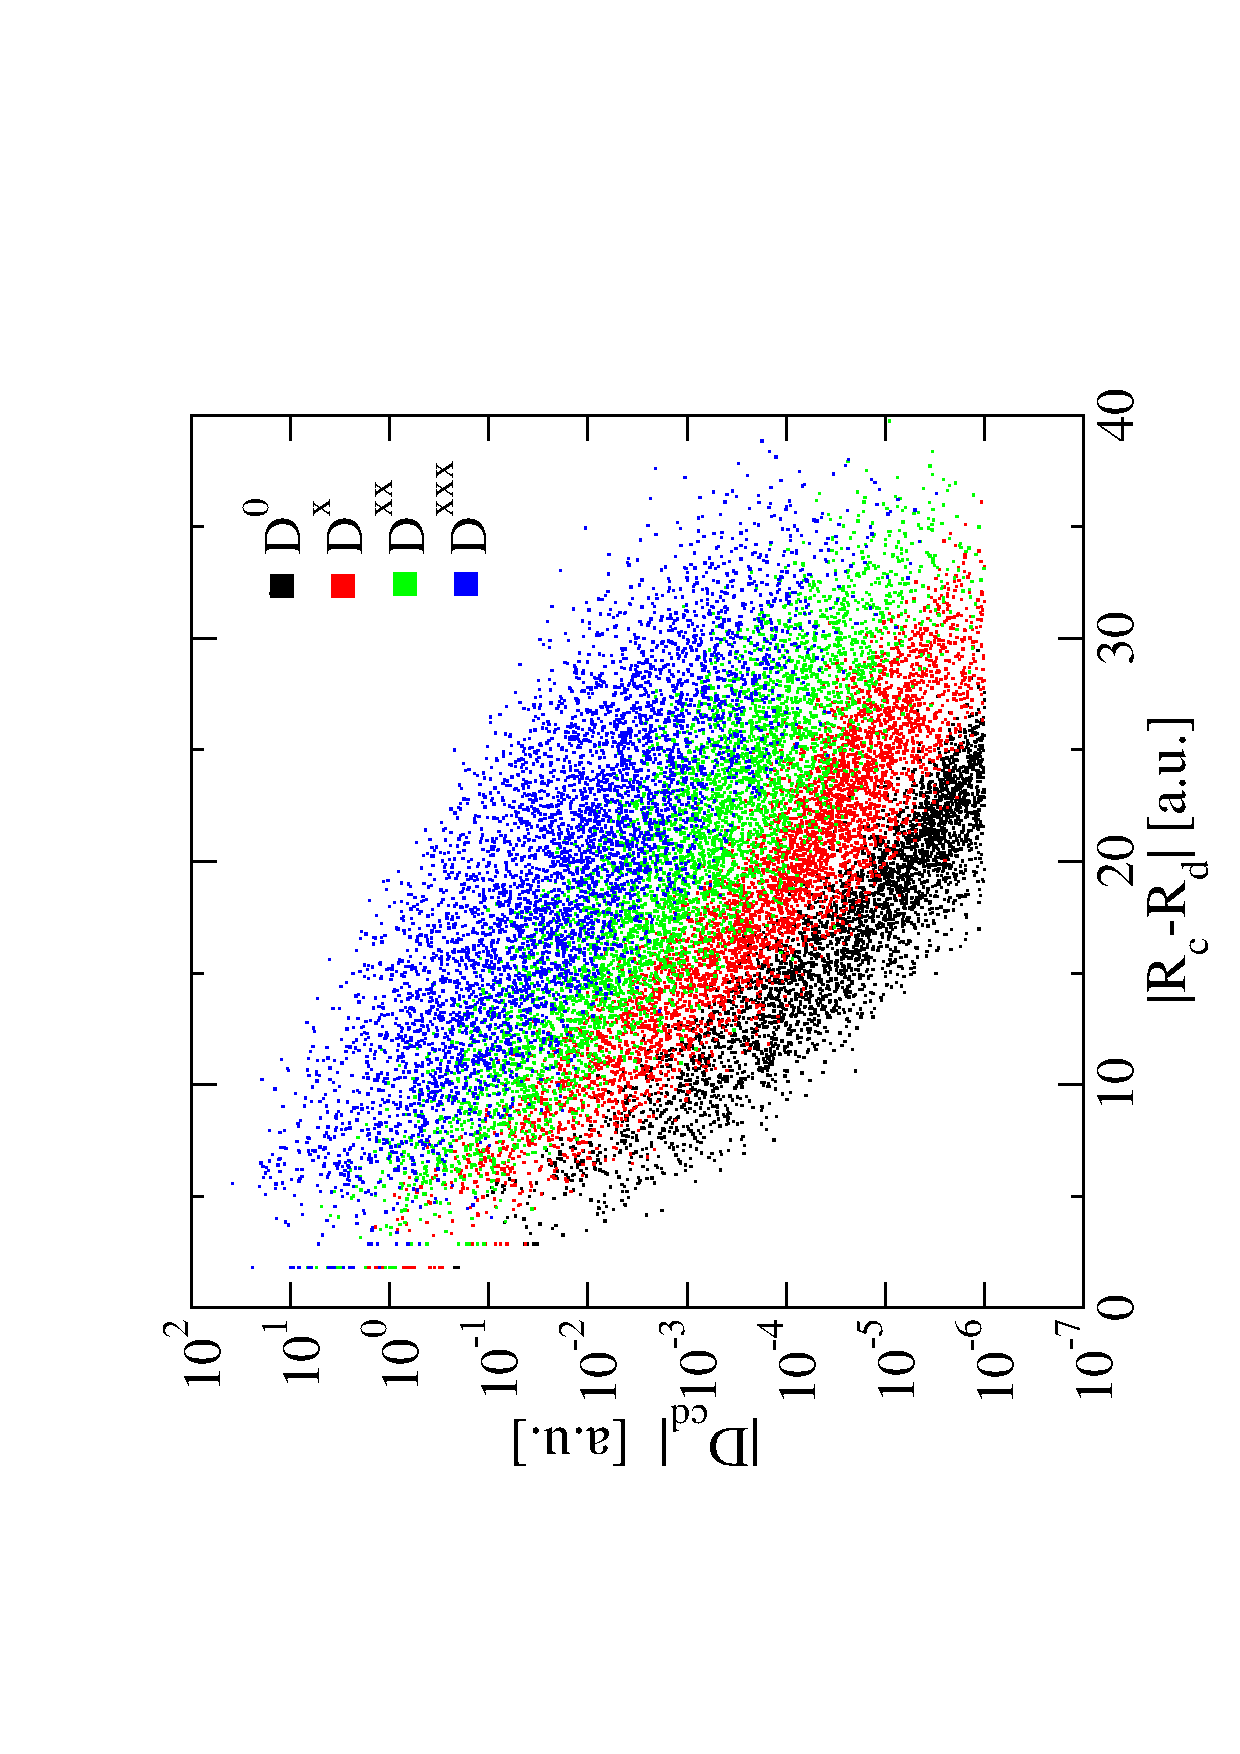
\includegraphics[angle=-90.00]{DMix_40pts}}
\end{figure}

%%%%%%%%%%%%%%%%%%%%%%%%%%%%%%%%%%%%%%%%%%%%%%%%%%%%%%%%%%%%%%%%
%%%%%%%%%%%%%%%%%%%%%%%%%%%%%%%%%%%%%%%%%%%%%%%%%%%%%%%%%%%%%%%%
\section{Summary and Conclusion}
 We have proposed and demonstrated a linear scaling self
 consistent scheme for high order response properties.
 The scheme solves the coupled perturbed self consistent field 
 equation by the perturbed projection method. We have also shown
 that the perturbed projection method can be expended to high
 order (e.g. up to 10-th order in the present paper).

We have presented a simple and efficient algorithm for solution 
of the coupled-perturbed self-consistent-field (CPSCF) equations 
in the context of spectral projection and static
electric polarizabilities. Unique features of the perturbed 
projection algorithm include linear scaling, simplicity, numerical 
stability and quadratic convergence in computation of the derivative
density matrices.

We have shown that the density matrix response is local 
upon {\em global} electric perturbation, corresponding to an approximate 
exponential decay of matrix elements. A similar exponential decay
in the first order response corresponding to the {\em local} nuclear 
displacement has previously been demonstrated by Ochsenfeld and 
Head-Gordon \cite{Ochsenfeld97}. These key observations are expected to
hold generally for both local and global perturbations to insulating systems.  
We note also that the method is not unique to the TC2 generator or 
{\sc MondoSCF} $N$-scaling algorithms, but can be straightforwardly 
extended to other purification schemes such as TRS4 \cite{ANiklasson03} as
well as other electronic structure programs.

Convergence of the CPSCF equations for these systems (water cluster ...)
are typically achieved in about 10 cycles, independent of cluster size, basis set,
matrix threshold or order of the response calculated.

The perturbed projectro algorithm described in steps (\ref{FockBuild}-\ref{DDeriv}) and 
(\ref{PP1}-\ref{PP2})
can be easily extended to the linear scaling computation of
DFT and hybrid DFT models and a large class of static molecular properties
such as the geometrical derivatives so important
in the evaluation of the nuclear hessian, the nuclear magnetic
shielding tensor (NMR shift), indirect spin-spin coupling and
electronic g-tensor.


%%%%%%%%%%%%%%%%%%%%%%%%%%%%%%%%%%%%%%%%%%%%%%%%%%%%%%%%%%%%%%%%
%%%%%%%%%%%%%%%%%%%%%%%%%%%%%%%%%%%%%%%%%%%%%%%%%%%%%%%%%%%%%%%%
%Acknowledgements
\begin{acknowledgments}
 This work has been supported by the US Department of Energy 
 under contract ???????????? and the ASCI project.  
 The Advanced Computing Laboratory of Los 
 Alamos National Laboratory is acknowledged.
 All the numerical computations have been
 performed on computing resources located at this facility.
\end{acknowledgments}
%%%%%%%%%%%%%%%%%%%%%%%%%%%%%%%%%%%%%%%%%%%%%%%%%%%%%%%%%%%%%%%%
%%%%%%%%%%%%%%%%%%%%%%%%%%%%%%%%%%%%%%%%%%%%%%%%%%%%%%%%%%%%%%%%
\bibliography{Response3}
%%%%%%%%%%%%%%%%%%%%%%%%%%%%%%%%%%%%%%%%%%%%%%%%%%%%%%%%%%%%%%%%
%%%%%%%%%%%%%%%%%%%%%%%%%%%%%%%%%%%%%%%%%%%%%%%%%%%%%%%%%%%%%%%%
%%%%%%%%%%%%%%%%%%%%%%%%%%%%%%%%%%%%%%%%%%%%%%%%%%%%%%%%%%%%%%%%
%%%%%%%%%%%%%%%%%%%%%%%%%%%%%%%%%%%%%%%%%%%%%%%%%%%%%%%%%%%%%%%%
%%%%%%%%%%%%%%%%%%%%%%%%%%%%%%%%%%%%%%%%%%%%%%%%%%%%%%%%%%%%%%%%
\end{document}
%
% ****** End of file apssamp.tex ******
